\documentclass[10pt]{beamer}
\usepackage{graphicx}
\usepackage{amsmath,amssymb,mathrsfs}
\usepackage{ushort}
%\usepackage{subfigure}
\usepackage{array,multicol,multirow}
\usepackage{rotating}
\usepackage{makecell}
\usepackage{moresize}
\usepackage{xcolor}
\usepackage{cmbright}
\usepackage{amsfonts}
%\usepackage{fontspec}
\usepackage{ulem}
\usepackage{epstopdf}
\usepackage{booktabs}
\usepackage{caption}
\usepackage{amsmath}
\usepackage{subcaption}
\usepackage{pifont}
\usetheme{default}
\beamertemplatenavigationsymbolsempty
\hypersetup{pdfpagemode=UseNone}

%\usefonttheme{professionalfonts}
\usefonttheme{serif}
% \usepackage[no-math]{fontspec}
%\setmainfont{HelveticaNeue-Light}

\setbeamersize{text margin left=0.5cm,text margin right=0.5cm}


\definecolor{gred}{RGB}{200,0,25}
\definecolor{gred2}{rgb}{0.8500,0.3250,0.0980}
%\definecolor{gblue}{RGB}{25,0,200}
\definecolor{gblue}{rgb}{0.0000,0.4470,0.7410}
\definecolor{ggreen}{RGB}{25,200,25}
\definecolor{gyel}{rgb}{0.9290,0.6940,0.1250}
\definecolor{dgreen}{rgb}{0,0.5,0}
\definecolor{gpink}{RGB}{255,0,247}
\definecolor{darkblue}{rgb}{0.0,0.0,0.8}

\definecolor{foreground}{RGB}{0,0,0}
\definecolor{background}{RGB}{255,255,255}
%\definecolor{title}{RGB}{37,47,141}
\definecolor{title}{RGB}{0,0,0}
%\definecolor{title}{RGB}{25,0,200}
\definecolor{gray}{RGB}{155,155,155}
%\definecolor{subtitle}{RGB}{128,128,128}
\definecolor{subtitle}{RGB}{0,0,0}
\definecolor{hilight}{RGB}{102,255,204}
\definecolor{vhilight}{RGB}{255,111,207}


\newcommand{\tw}{\textcolor{white} }
\newcommand{\tblk}{\textcolor{black} }
\newcommand<>\tr{\textcolor#1{gred}}
\newcommand<>\trb[1]{\textcolor#2{gred}{\textbf#2{#1}}}
\newcommand<>\trrb[1]{\textcolor#2{gred2}{\textbf#2{#1}}}
\newcommand<>\tyb[1]{\textcolor#2{gyel}{\textbf#2{#1}}}
\newcommand<>\tbb[1]{\textcolor#2{gblue}{\textbf#2{#1}}}
\newcommand{\tb}{\textcolor{gblue} }
\newcommand{\tg}{\textcolor{dgreen} }
\newcommand{\tp}{\textcolor{gpink} }

\setbeamercolor{titlelike}{fg=title}
\setbeamercolor{subtitle}{fg=subtitle}
\setbeamercolor{institute}{fg=foreground}
\setbeamercolor{normal text}{fg=foreground,bg=background}

%% underline frame title
\setbeamertemplate{frametitle}
{
\vspace{0.3cm}
%  \textcolor[rgb]{0.0,0.5,0.8}{\Huge \underline{\Large \textcolor[rgb]{0.35,0.35,0.35}{\insertframetitle}}}
\insertframetitle \\
\noindent \hspace{-0.2cm} \rule{12cm}{0.6pt} \vspace{-0.5cm}
}


\setbeamercolor{item}{fg=foreground} % color of bullets
\setbeamercolor{subitem}{fg=foreground}
\setbeamercolor{subsubitem}{fg=foreground}
\setbeamercolor{itemize/enumerate subbody}{fg=foreground}
\setbeamertemplate{itemize item}[circle]
\setbeamertemplate{itemize subitem}[circle]
\setbeamertemplate{itemize subsubitem}[circle]
\setbeamerfont{itemize/enumerate subbody}{size=\normalsize}
\setbeamerfont{itemize/enumerate subitem}{size=\normalsize}
\setbeamerfont{itemize/enumerate subsubitem}{size=\normalsize}

%% slide numbers in bottom right
\setbeamertemplate{footline}{%
    \raisebox{5pt}{\makebox[\paperwidth]{\hfill\makebox[20pt]{\color{gray}
          \scriptsize\insertframenumber}}}\hspace*{5pt}}

\newcommand{\bi}{\begin{itemize}}
\newcommand{\ei}{\end{itemize}}
\newcommand{\be}{\begin{enumerate}}
\newcommand{\ee}{\end{enumerate}}
\newcommand{\bd}{\begin{description}}
\newcommand{\ed}{\end{description}}
\newcommand{\ig}{\includegraphics}
\newcommand{\bs}{\begin{frame}}
\newcommand{\es}{\end{frame}}
%\newcommand{\st}{\frametitle}
\newcommand{\subt}[1]{{\footnotesize \color{subtitle} {#1}}}

\newcommand{\R}{{\mathbb R}}
\newcommand{\Q}{{\mathbb Q}}
\newcommand{\Z}{{\mathbb Z}}
\newcommand{\N}{{\mathbb N}}
\newcommand{\Po}{{\mathbb P}}
\newcommand{\M}{{\mathcal M}}
\newcommand{\A}{{\mathcal A}}
\newcommand{\RR}{\mathbb{R}}
%\newtheorem{assum}[theorem]{Assumption}
\newtheorem{assumption}[theorem]{Assumption}
\newtheorem{proposition}{Proposition}
\newtheorem{defn}[theorem]{Definition}

%%%%%%%%%%%%%%%%%%%%%%%%%%%%%%%%%%%%%%%%%%%%%%%%%%%%%%%%%%%%%%%%%%%%%%%%%
% Chicago Manual of Style Tables package
\usepackage{booktabs}
\usepackage{multicol}
\usepackage{multirow}
\usepackage[flushleft]{threeparttable}
%\usepackage{tablenotes}
% Create the control over the stretch between the arrays command
\newcommand{\ra}[1]{\renewcommand{\arraystretch}{#1}}
\newcommand\TopStr{\rule{0pt}{3.0ex}}       % Top strut
%%%%%%%%%%%%%%%%%%%%%%%%%%%%%%%%%%%%%%%%%%%%%%%%%%%%%%%%%%%%%%%%%%%%%%%%%


%\captionsetup[subfigure]{labelformat=empty}

%\renewcommand\thesubfigure{\Alph{subfigure}}


\begin{document}

\title[International Attitudes Toward Global Policies]{International Attitudes Toward Global Policies \vspace{1ex}}

\author{Adrien Fabre \qquad Thomas Douenne \qquad Linus Mattauch \vspace{-1ex}}

\institute{CNRS, Cired \qquad \quad University of Amsterdam\qquad \quad TU Berlin, Oxford\vspace{3ex}}


\date{Leiden University\\[1ex] September 2023}

\begin{frame}[noframenumbering,plain]
\maketitle

\end{frame}

%%%%%%%%%%%%%%%%%%%%%%%%%%%%%%%%%%%%%%%%%%%%%%%%%%%%%%%%%%%%%%%%%%
\section{Introduction}
%%%%%%%%%%%%%%%%%%%%%%%%%%%%%%%%%%%%%%%%%%%%%%%%%%%%%%%%%%%%%%%%%%

\begin{frame}
\frametitle{Motivation}

\begin{itemize}
\setlength\itemsep{0.3cm}
    \item Two major global challenges: extreme poverty and climate change.
    
    \item Climate change: some worrying trends:
    \begin{itemize}
        \item[\ding{226}] Without a strengthening of policies, global warming of 3.2\textdegree C projected by 2100 (\textcolor{blue}{IPCC, 2023}).

        \item[\ding{226}] At these temperatures (and even far below), major changes to ecosystems, and major impacts on humans.
    \end{itemize}

    \item Extreme poverty: still a very bleak picture:
    \begin{itemize}
        \item[\ding{226}] Around 700 million people live with less than \$2/day.
    \end{itemize}

    \pause

    \item Both issues are linked:
    \begin{itemize}
        \item[\ding{226}] climate change expected to impact differently (typically more) people in extreme poverty;

        \item[\ding{226}] deciding on climate policy requires to decide on burden sharing rules.
    \end{itemize}

\end{itemize}

\end{frame}
\begin{frame}
\frametitle{Research question}

\begin{itemize}
\setlength\itemsep{0.3cm}
    \item Global problems, ``require'' international/global coordination.

    \item Free rider problem: countries have incentives to shirk and let others fix these problems.

    \pause

    \item Still, growing number of unilateral initiatives to combat climate change over the world: many people/countries are actually willing to act!
    
    \item Rapid and effective action implies significant costs for high-income countries as 1) they cause more pollution and 2) have more resources to address these problems.
\end{itemize}

\vspace{0.5cm}
\pause

$\Rightarrow$ \textbf{Questions: Are citizens around the world willing to coordinate on these policies? Are citizens in high-income countries willing to make sacrifices to address climate change and extreme poverty?}

\end{frame}
\begin{frame}
\frametitle{What we do}

\begin{itemize}
\setlength\itemsep{0.5cm}
    \item We study attitudes towards global policies to combat climate change and extreme poverty;
    \begin{itemize}
        \item[\ding{226}] we use survey data from 20 high- and middle-income countries and >40k respondents from \textcolor{blue}{Dechezleprêtre et al. (2022)};
        \item[\ding{226}] we run complementary surveys on 8k respondents in the US, UK, Germany, France, and Spain.
    \end{itemize}

    \item We examine the sincerity of support for these policies;
    \begin{itemize}
        \item[\ding{226}] We focus on a specific global redistributive climate policy: the ``Global Climate Scheme''.
        \item[\ding{226}] We rely on diverse methods, e.g. list experiment, conjoint analysis, petition, prioritization exercise.
    \end{itemize}

    % \item We reflect on the reasons behind the absence of policy implementation.
\end{itemize}

\end{frame}
\begin{frame}
\frametitle{What we find}

\begin{itemize}
\setlength\itemsep{0.5cm}
    \item We find strong support for global redistributive and climate policies all over the world, including:
    \begin{itemize}
        \item[\ding{226}] a global carbon budget with tradable country shares;
        \item[\ding{226}] a tax on millionaires to finance low-income countries;
        \item[\ding{226}] a global democratic assembly on climate change;
        \item[\ding{226}] etc.
    \end{itemize}

    \item Focusing on high-income countries (who would pay the burden of these policies) we confirm that support is mostly sincere.
\end{itemize}

\vspace{0.8cm}
\pause

$\Rightarrow$ These results raise questions about the reasons behind lack of policy implementation. If not lack of demand, is there an issue with the supply?

\end{frame}
\begin{frame}
\frametitle{Related work}

\begin{itemize}
\setlength\itemsep{0.3cm}
    \item Prior literature uses surveys to study attitudes towards climate change and climate policies (see e.g., \textcolor{blue}{Whitmarsh \& Capstick, 2018}; \textcolor{blue}{Douenne \& Fabre, 2020}; \textcolor{blue}{Dechezleprêtre et al., 2022}).

    \item Also large literature on preferences for (national) redistribution (see \textcolor{blue}{Mengel \& Weidenholzer, 2022}).

    \pause

    \item Literature using attitudinal surveys to study preferences for \textit{global} redistribution is more scarce:
    \begin{itemize}
    \setlength\itemsep{0.15cm}
        \item[\ding{226}] \textcolor{blue}{Carattini et al. (2019)}: study global carbon taxes with international per capita redistribution.

        \item[\ding{226}] \textcolor{blue}{Fehr et al (2022)}: study people's perception of their rank in the global income distribution and their preferences to redistribute.

        \item[\ding{226}] \textcolor{blue}{Ghassim et al. (2022)}: study support for global democracy.
    \end{itemize}
\end{itemize}

\vspace{0.3cm}
\pause

\textbf{Our contribution:} investigate large panel of global policies across many countries and respondentss, and test sincerity.

\end{frame}

\section{Data}

\begin{frame}[noframenumbering,plain]
\begin{center}
\huge Survey data
\end{center}
\end{frame}


% \begin{frame}
% \frametitle{Data collection: overview (1/3)}

% [Text]% Explain surveys, the OECD one and the complementary ones. Explain their coverage, their goals, their sample size, their respective representativity, etc.

% % company Bilendi // online survey // representative according to some quotas // 


% \end{frame}
\begin{frame}
\frametitle{Data collection: overview (1/2)}

\begin{itemize}
    \item Study based on two sets of online surveys:
\end{itemize}

\begin{table}[h!]
\renewcommand{\arraystretch}{1.5}
\caption{Summary of the surveys used in the analysis.}
\label{tab:survey_summary}
\centering
\footnotesize
\begin{tabular}{ |p{1.3cm}|p{2.5cm}|p{1.3cm}|p{1.3cm}|p{2.0cm}|  }
\cline{2-5}
\multicolumn{1}{c|}{} & \textbf{Global survey} & \multicolumn{3}{|c|}{\textbf{Complementary surveys}} \\
\hline
\textbf{\textit{Name}} & \textit{Global} & \textit{US1} & \textit{US2} & \textit{Eu} \\
\hline
\textbf{Region} & 20 high and middle-income countries & U.S. & U.S. & France, Germany, Spain, U.K. \\
\hline
\textbf{Sample size} & 40,680 & 3,000 & 2,000 & 3,000 \\
\hline
\textbf{Main purpose} & Stated support for global policies & \multicolumn{3}{|p{4.6cm}|}{Focus on GCS (sincerity, rationales, etc.) + Support for global redistribution + Universalistic values} \\
\hline
\end{tabular}
\end{table}

\end{frame}
\begin{frame}
\frametitle{Data collection: overview (2/2)}

\begin{figure}
    \centering
    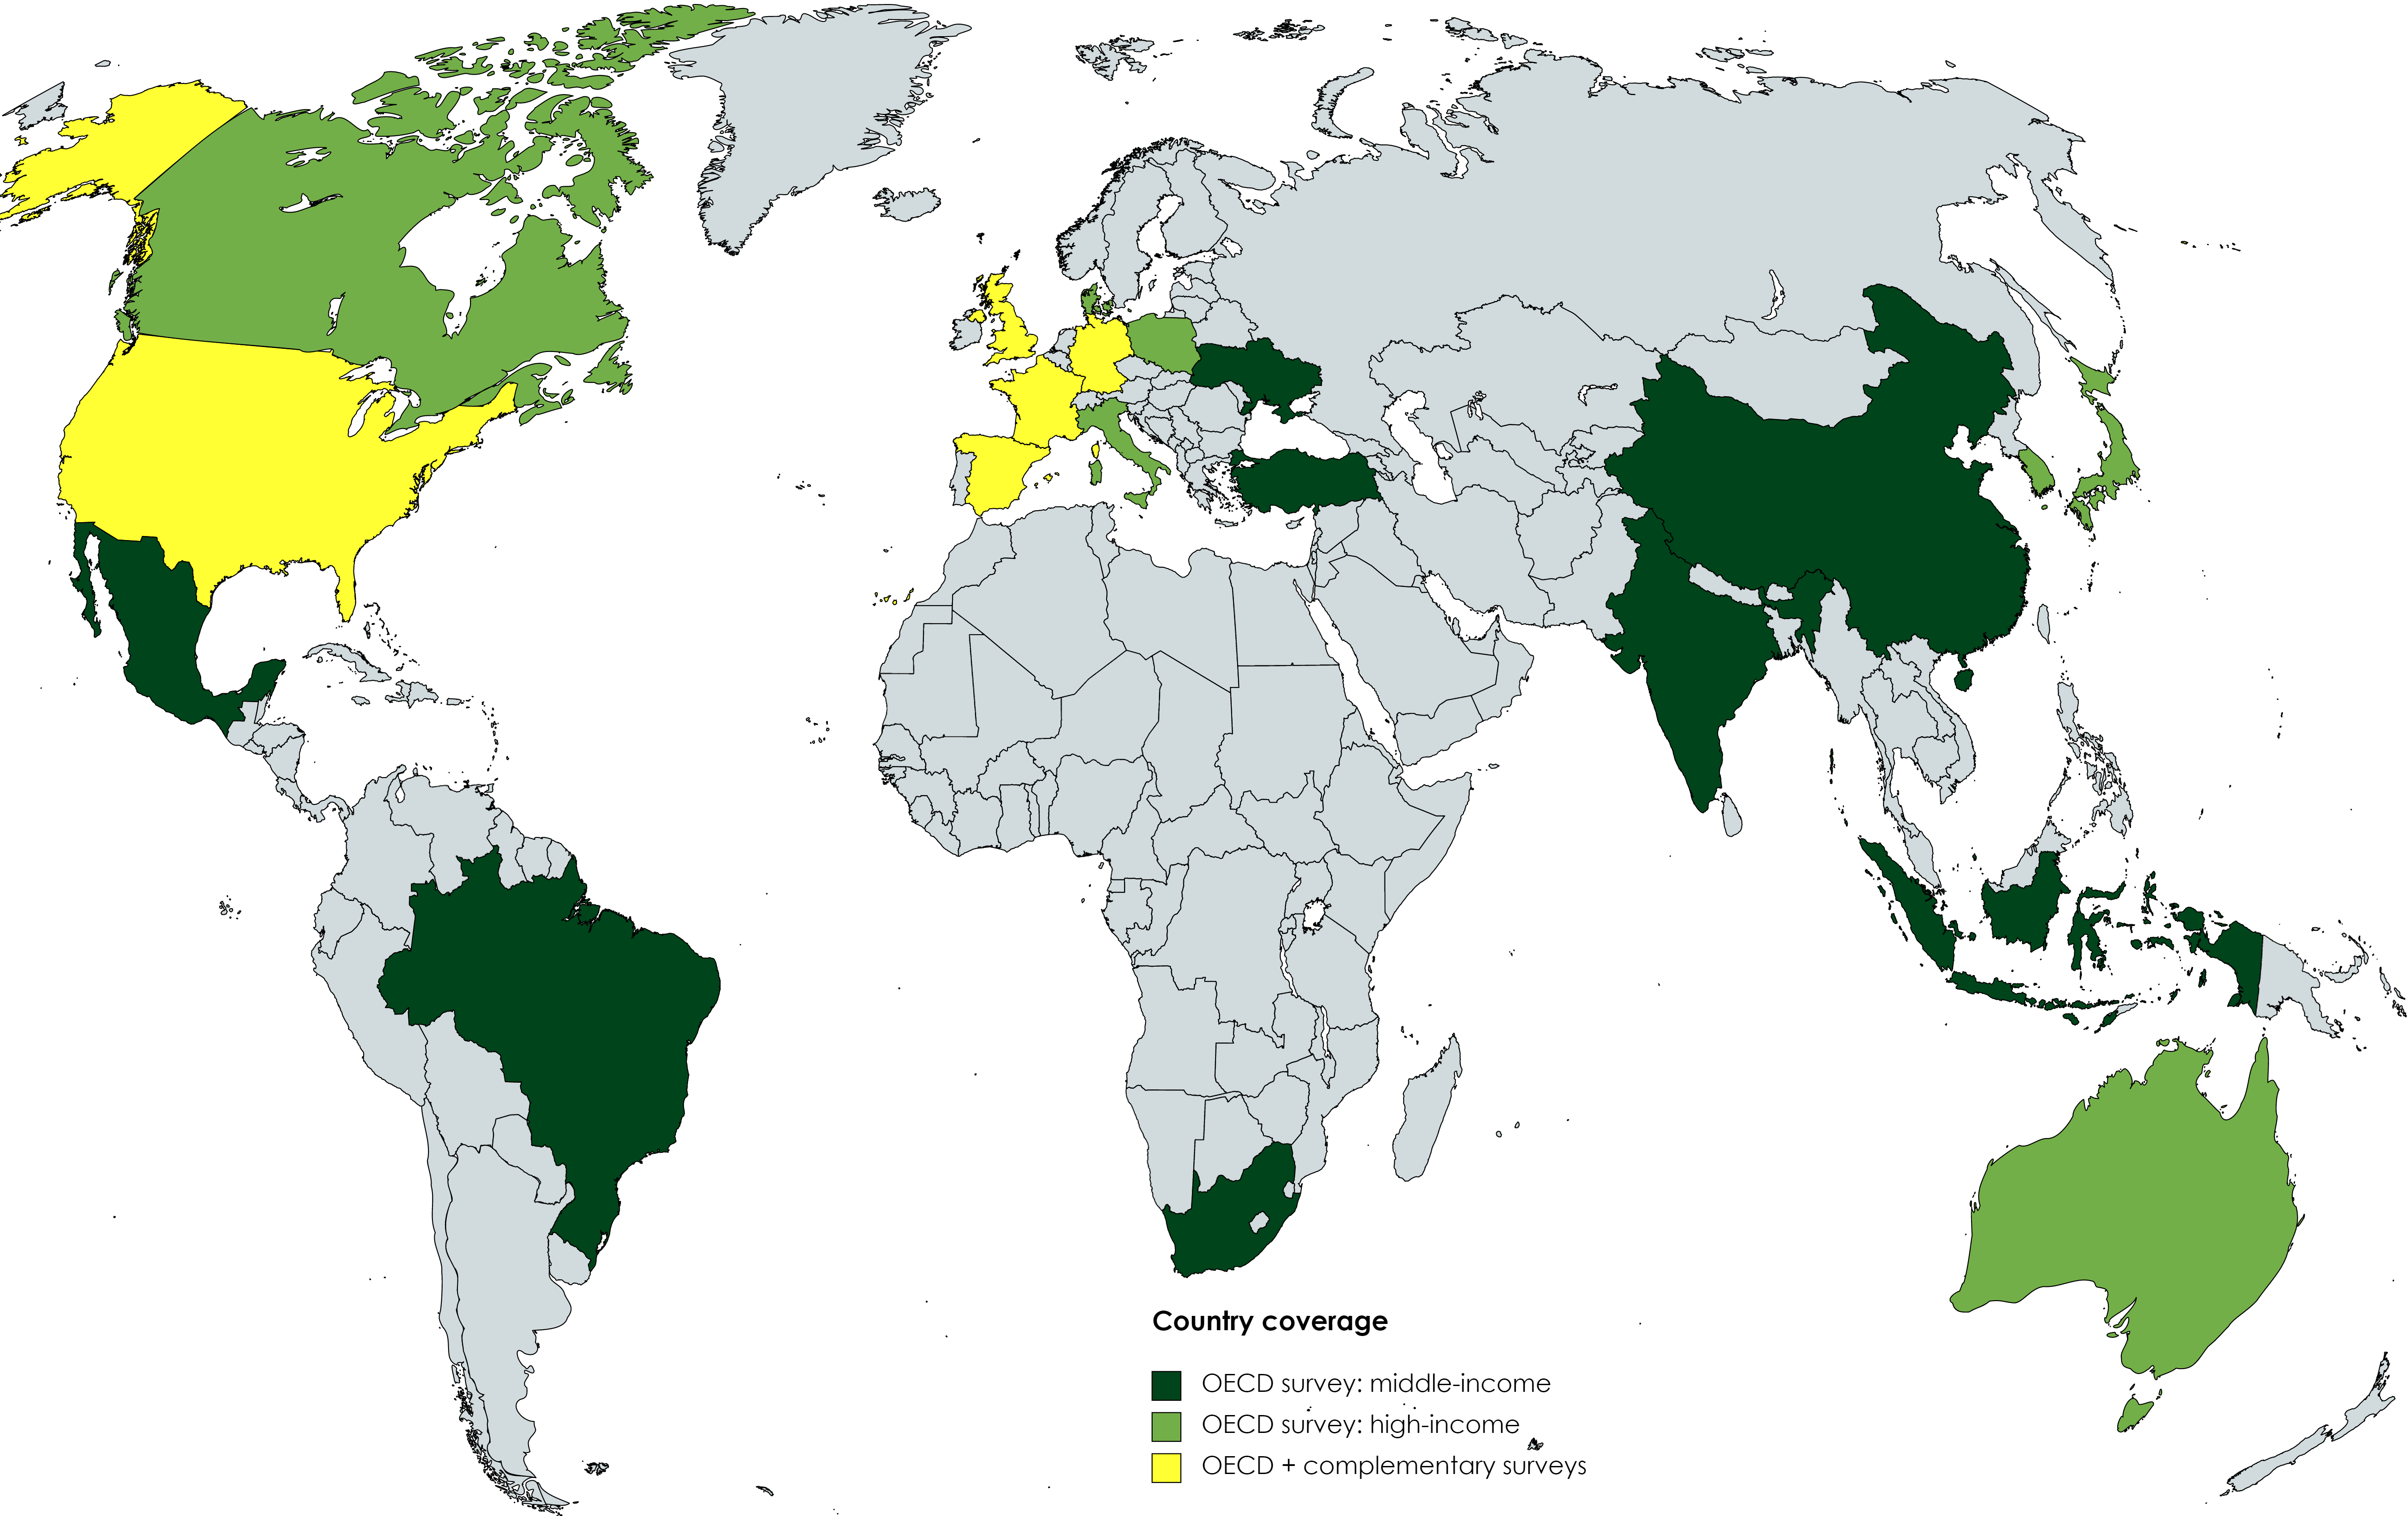
\includegraphics[width=0.85\textwidth]{../figures/maps/country_coverage.png}
    \caption{Country coverage of the surveys}
    \label{fig:enter-label}
\end{figure}

%TOSAY: mention also how it is collected, etc. Mention lenght of the surveys. Mention their representativity. Say that the global survey is used for another study, so it is actually longer.

\end{frame}
\begin{frame}

\begin{table}[h!]
    \caption[Sample representativeness of US1, US2, Eu]{Sample representativeness of the complementary surveys.}\label{tab:representativeness_waves}\vspace{-0.6cm}
    \makebox[\textwidth][c]{
        \resizebox*{!}{.95\textheight}{% 73 without notes cf. https://tex.stackexchange.com/questions/13809/resizing-a-table-by-textheight 
        
\begin{tabular}[t]{llllllllll}
\toprule
\multicolumn{1}{c}{} & \multicolumn{3}{c}{US1} & \multicolumn{3}{c}{US2} & \multicolumn{3}{c}{EU} \\
\cmidrule(l{3pt}r{3pt}){2-4} \cmidrule(l{3pt}r{3pt}){5-7} \cmidrule(l{3pt}r{3pt}){8-10}
  & Pop. & Sample & \makecell{Weighted\\sample} & Pop. & Sample & \makecell{Weighted\\sample} & Pop. & Sample & \makecell{Weighted\\sample}\\
\midrule
Sample size &  & 3,000 & 3,000 &  & 516 & 516 &  & 2,979 & 2,979\\
\addlinespace
Gender: Woman & 0.51 & 0.52 & 0.51 & 0.51 & 0.65 & 0.56 & 0.51 & 0.49 & 0.51\\
Gender: Man & 0.49 & 0.47 & 0.49 & 0.49 & 0.34 & 0.44 & 0.49 & 0.51 & 0.49\\
\addlinespace
Income\_quartile: 1 & 0.25 & 0.27 & 0.25 & 0.25 & 0.53 & 0.35 & 0.25 & 0.28 & 0.25\\
Income\_quartile: 2 & 0.25 & 0.24 & 0.25 & 0.25 & 0.31 & 0.31 & 0.25 & 0.23 & 0.25\\
Income\_quartile: 3 & 0.25 & 0.25 & 0.25 & 0.25 & 0.13 & 0.23 & 0.25 & 0.25 & 0.25\\
Income\_quartile: 4 & 0.25 & 0.23 & 0.25 & 0.25 & 0.04 & 0.11 & 0.25 & 0.24 & 0.25\\
\addlinespace
Age: 18-24 & 0.12 & 0.12 & 0.12 & 0.12 & 0.09 & 0.11 & 0.10 & 0.11 & 0.10\\
Age: 25-34 & 0.18 & 0.15 & 0.18 & 0.18 & 0.19 & 0.19 & 0.15 & 0.17 & 0.15\\
Age: 35-49 & 0.24 & 0.25 & 0.24 & 0.24 & 0.29 & 0.25 & 0.24 & 0.25 & 0.24\\
Age: 50-64 & 0.25 & 0.27 & 0.25 & 0.25 & 0.27 & 0.27 & 0.26 & 0.25 & 0.26\\
Age: 65+ & 0.21 & 0.21 & 0.21 & 0.21 & 0.16 & 0.18 & 0.25 & 0.23 & 0.25\\
\addlinespace
Diploma\_25\_64: Below upper secondary & 0.06 & 0.02 & 0.05 & 0.06 & 0.06 & 0.06 & 0.13 & 0.14 & 0.13\\
Diploma\_25\_64: Upper secondary & 0.28 & 0.25 & 0.28 & 0.28 & 0.41 & 0.33 & 0.23 & 0.19 & 0.23\\
Diploma\_25\_64: Post secondary & 0.34 & 0.40 & 0.34 & 0.34 & 0.30 & 0.32 & 0.29 & 0.33 & 0.29\\
\addlinespace
Race: White only & 0.60 & 0.67 & 0.61 & 0.60 & 0.14 & 0.40 &  &  & \\
Race: Hispanic & 0.18 & 0.15 & 0.19 & 0.18 & 0.46 & 0.30 &  &  & \\
Race: Black & 0.13 & 0.16 & 0.14 & 0.13 & 0.37 & 0.22 &  &  & \\
\addlinespace
Region: Northeast & 0.17 & 0.20 & 0.17 & 0.17 & 0.16 & 0.18 &  &  & \\
Region: Midwest & 0.21 & 0.22 & 0.21 & 0.21 & 0.15 & 0.19 &  &  & \\
Region: South & 0.38 & 0.39 & 0.38 & 0.38 & 0.47 & 0.45 &  &  & \\
Region: West & 0.24 & 0.20 & 0.24 & 0.24 & 0.22 & 0.18 &  &  & \\
\addlinespace
Urban: TRUE & 0.73 & 0.78 & 0.74 & 0.73 & 0.83 & 0.74 &  &  & \\
\addlinespace
Employment\_18\_64: Inactive & 0.20 & 0.16 & 0.16 & 0.20 & 0.19 & 0.15 & 0.17 & 0.15 & 0.15\\
Employment\_18\_64: Unemployed & 0.02 & 0.07 & 0.08 & 0.02 & 0.15 & 0.11 & 0.03 & 0.05 & 0.05\\
\addlinespace
Vote: Left & 0.32 & 0.47 & 0.45 & 0.32 & 0.53 & 0.48 & 0.30 & 0.32 & 0.32\\
Vote: Center-right or Right & 0.30 & 0.31 & 0.31 & 0.30 & 0.15 & 0.23 & 0.28 & 0.32 & 0.32\\
Vote: Far right &  &  &  &  &  &  & 0.10 & 0.10 & 0.10\\
\addlinespace
Country: FR &  &  &  &  &  &  & 0.24 & 0.24 & 0.24\\
Country: DE &  &  &  &  &  &  & 0.33 & 0.33 & 0.33\\
Country: ES &  &  &  &  &  &  & 0.18 & 0.18 & 0.18\\
Country: UK &  &  &  &  &  &  & 0.25 & 0.25 & 0.25\\
\addlinespace
Urbanity: Cities &  &  &  &  &  &  & 0.43 & 0.49 & 0.43\\
Urbanity: Towns and suburbs &  &  &  &  &  &  & 0.33 & 0.32 & 0.33\\
Urbanity: Rural &  &  &  &  &  &  & 0.25 & 0.19 & 0.25\\
\bottomrule
\end{tabular}
        }
    }
\end{table}
    
\end{frame}


\section{Stated support}


\begin{frame}[noframenumbering,plain]
\begin{center}
\huge Stated support
\end{center}
\end{frame}

% \begin{frame}
% \frametitle{Support: global survey (1/2)}

% \begin{figure}[h!]
%   \caption[Relative support for global climate policies]{Relative support for global climate policies.}
%   \vspace{-0.3cm}
%   \makebox[1.0\textwidth][c]{\includegraphics[width=1.0\textwidth]
%   {Images/figure_1_paper_gcs.png}}\label{fig:oecd}
%   \vspace{-0.3cm}
%   % {\footnotesize \\ $\quad$ \\ Note 1: The numbers represent the share of \textit{Somewhat} or \textit{Strongly support} among non-\textit{indifferent} answers (in percent, $n$ = 40,680).} 
% \end{figure}

% \end{frame}
\begin{frame}
\frametitle{Stated support: global survey (1/3)}

\begin{itemize}
    \item Question: ``At which level(s) do you think public policies to tackle climate change need to be put in place?''
\end{itemize}

    \pause

\begin{figure}[h!]
  \caption[Appropriate scale for climate policies]{Appropriate scale for climate policies.}
  \vspace{-0.3cm}
  \makebox[1.0\textwidth][c]{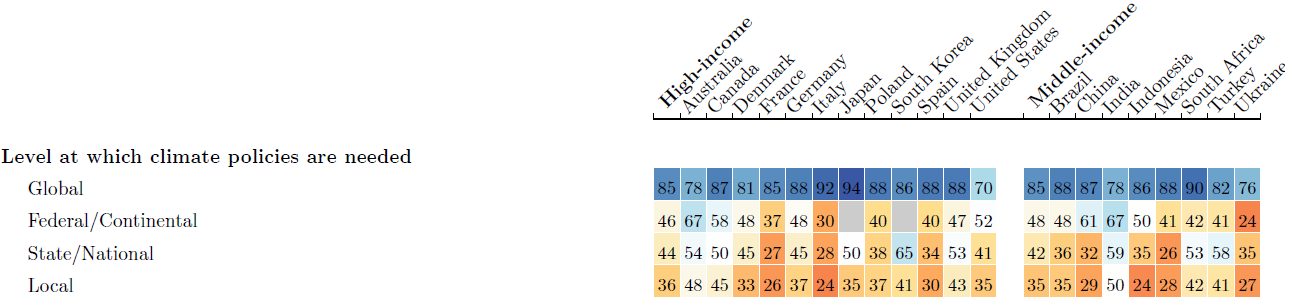
\includegraphics[width=1.0\textwidth]
  {../figures/OECD/Heatmap_scale.png}}\label{fig:oecd}
  \vspace{-0.4cm}
  % {\scriptsize \\ $\quad$ \\ Note: The numbers represent the share of \textit{Somewhat} or \textit{Strongly support} among non-\textit{indifferent} answers (in percent, $n$ = 40,680).} 
\end{figure}

\begin{itemize}
    \item[\ding{226}] Very large majority favors the global level, more local approaches are less supported.
    \item[\ding{226}] Consistent with people caring about fairness and effectiveness of climate policies.
\end{itemize}


\end{frame}
\begin{frame}
\frametitle{Stated support: global survey (2/3)}\label{slide_global_support}

\begin{itemize}
    \item We ask support for four climate policies:  \hyperlink{slide_wording}{\beamergotobutton{See wording}}
\end{itemize}

    \pause

\begin{figure}[h!]
  \caption[Relative support for global climate policies]{Relative support for global climate policies.}
  \vspace{-0.3cm}
  \makebox[1.0\textwidth][c]{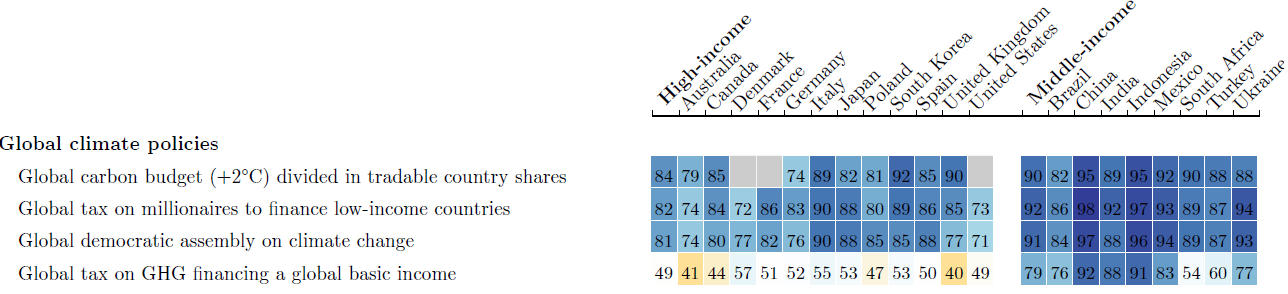
\includegraphics[width=1.0\textwidth]
  {../figures/OECD/Heatmap_global_policies.png}}\label{fig:oecd}
  \vspace{-0.4cm}
  % {\scriptsize \\ $\quad$ \\ Note: The numbers represent the share of \textit{Somewhat} or \textit{Strongly support} among non-\textit{indifferent} answers (in percent, $n$ = 40,680).} 
\end{figure}

\vspace{0.2cm}

\begin{itemize}
    \item[\ding{226}] Three of them garner support in all countries, only the carbon tax does not receive majority support everywhere.
\end{itemize}

\end{frame}
\begin{frame}
\frametitle{Stated support: global survey (3/3)}

\begin{itemize}
    \item Preferred allocation rule for tradable pollution quotas:
\end{itemize}

    \pause

\begin{figure}[h!]
  \caption[Preferred burden sharing rule]{Preferred burden sharing rule.}
  \vspace{-0.3cm}
  \makebox[1.0\textwidth][c]{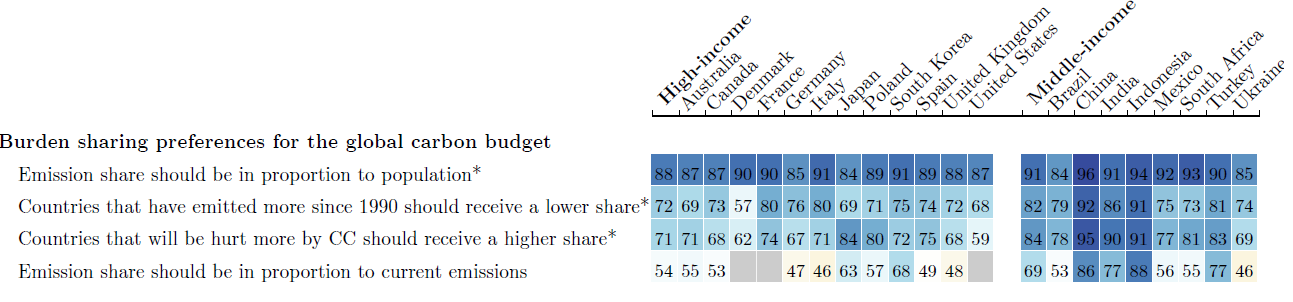
\includegraphics[width=1.0\textwidth]
  {../figures/OECD/Heatmap_burden-sharing.png}}\label{fig:oecd}
  \vspace{-0.4cm}
  % {\scriptsize \\ $\quad$ \\ Note: The numbers represent the share of \textit{Somewhat} or \textit{Strongly support} among non-\textit{indifferent} answers (in percent, $n$ = 40,680).} 
\end{figure}

\begin{itemize}
    \item[\ding{226}] equal per capita allocation is the preferred option, virtually consensual;

    \item[\ding{226}] taking into account historical responsibility or vulnerability to climate change also largely supported;
    
    \item[\ding{226}] grandfathering (i.e., prop. to current emissions) least supported.
\end{itemize}

\end{frame}
\begin{frame}
\frametitle{Inconsistent support for carbon taxation?}

Two contrasting results:

\vspace{0.2cm}

\begin{enumerate}
\setlength\itemsep{0.2cm}
    \item People are largely in favor of a carbon budget with tradable quotas, even more so if quotas are allocated on an equal per capita basis.
    
    \item People are less in favor of a global carbon tax financing a basic income.
\end{enumerate}

\vspace{0.2cm}
\pause

$\Rightarrow$ Yet, in theory these two policies amount to the same thing (same distributional outcomes). Is that inconsistent?

\pause
\vspace{0.6cm}

Possible explanations:

\vspace{0.1cm}

\begin{itemize}
    \item[\ding{226}] lower expected environmental effectiveness of the tax;
    \item[\ding{226}] distributional effects more salient with the tax;
    \item[\ding{226}] a form of tax aversion?
\end{itemize}

\end{frame}
\begin{frame}
\frametitle{Stated support: complementary surveys}

In the complementary surveys, we again enquire about support for many climate and redistributive policies:

\vspace{0.2cm}

\begin{itemize}
\setlength\itemsep{0.3cm}
    \item Multiple questions on wealth taxation;
    \item Multiple questions on foreign aid;
    \item Questions on global institutions, rules applying on trade tariffs, etc.
    \item In addition, specific focus on a ``Global Climate Scheme'' (GCS).
\end{itemize}

\vspace{0.5cm}
\pause

$\Rightarrow$ Again very high level of support for these policies.

\end{frame}
\begin{frame}
\frametitle{GCS: presentation (1/3)}

The Global Climate Scheme works as follows:

\vspace{0.05cm}

\begin{itemize}
\setlength\itemsep{0.15cm}
    \item Implements a cap on carbon emissions to limit global warming below 2\textdegree C.
    
    \item Emission rights are auctioned each year to polluting firms.

    \item Revenue is used to fund a global basic income, alleviating extreme poverty.
\end{itemize}

\vspace{0.4cm}
\pause

Specifically:

\vspace{0.05cm}

\begin{itemize}
\setlength\itemsep{0.15cm}
    \item Calibrated based on price and emissions trajectories from \textcolor{blue}{Stern \& Stiglitz (2017)}: \$90/tCO2 in 2030, from which we estimate that the basic income would amount to \$30 per month for each human above 15.
\end{itemize}

\vspace{0.4cm}
\pause

$\Rightarrow$ Again, same distributional effects as a global carbon tax financing a global basic income, and same as tradable quotas allocated on a per capita basis.

\end{frame}
\begin{frame}
\frametitle{GCS: presentation (2/3)}
    \begin{figure}
        \centering 
        \caption{Distributive effects of the Global Climate Scheme in 2030.}
        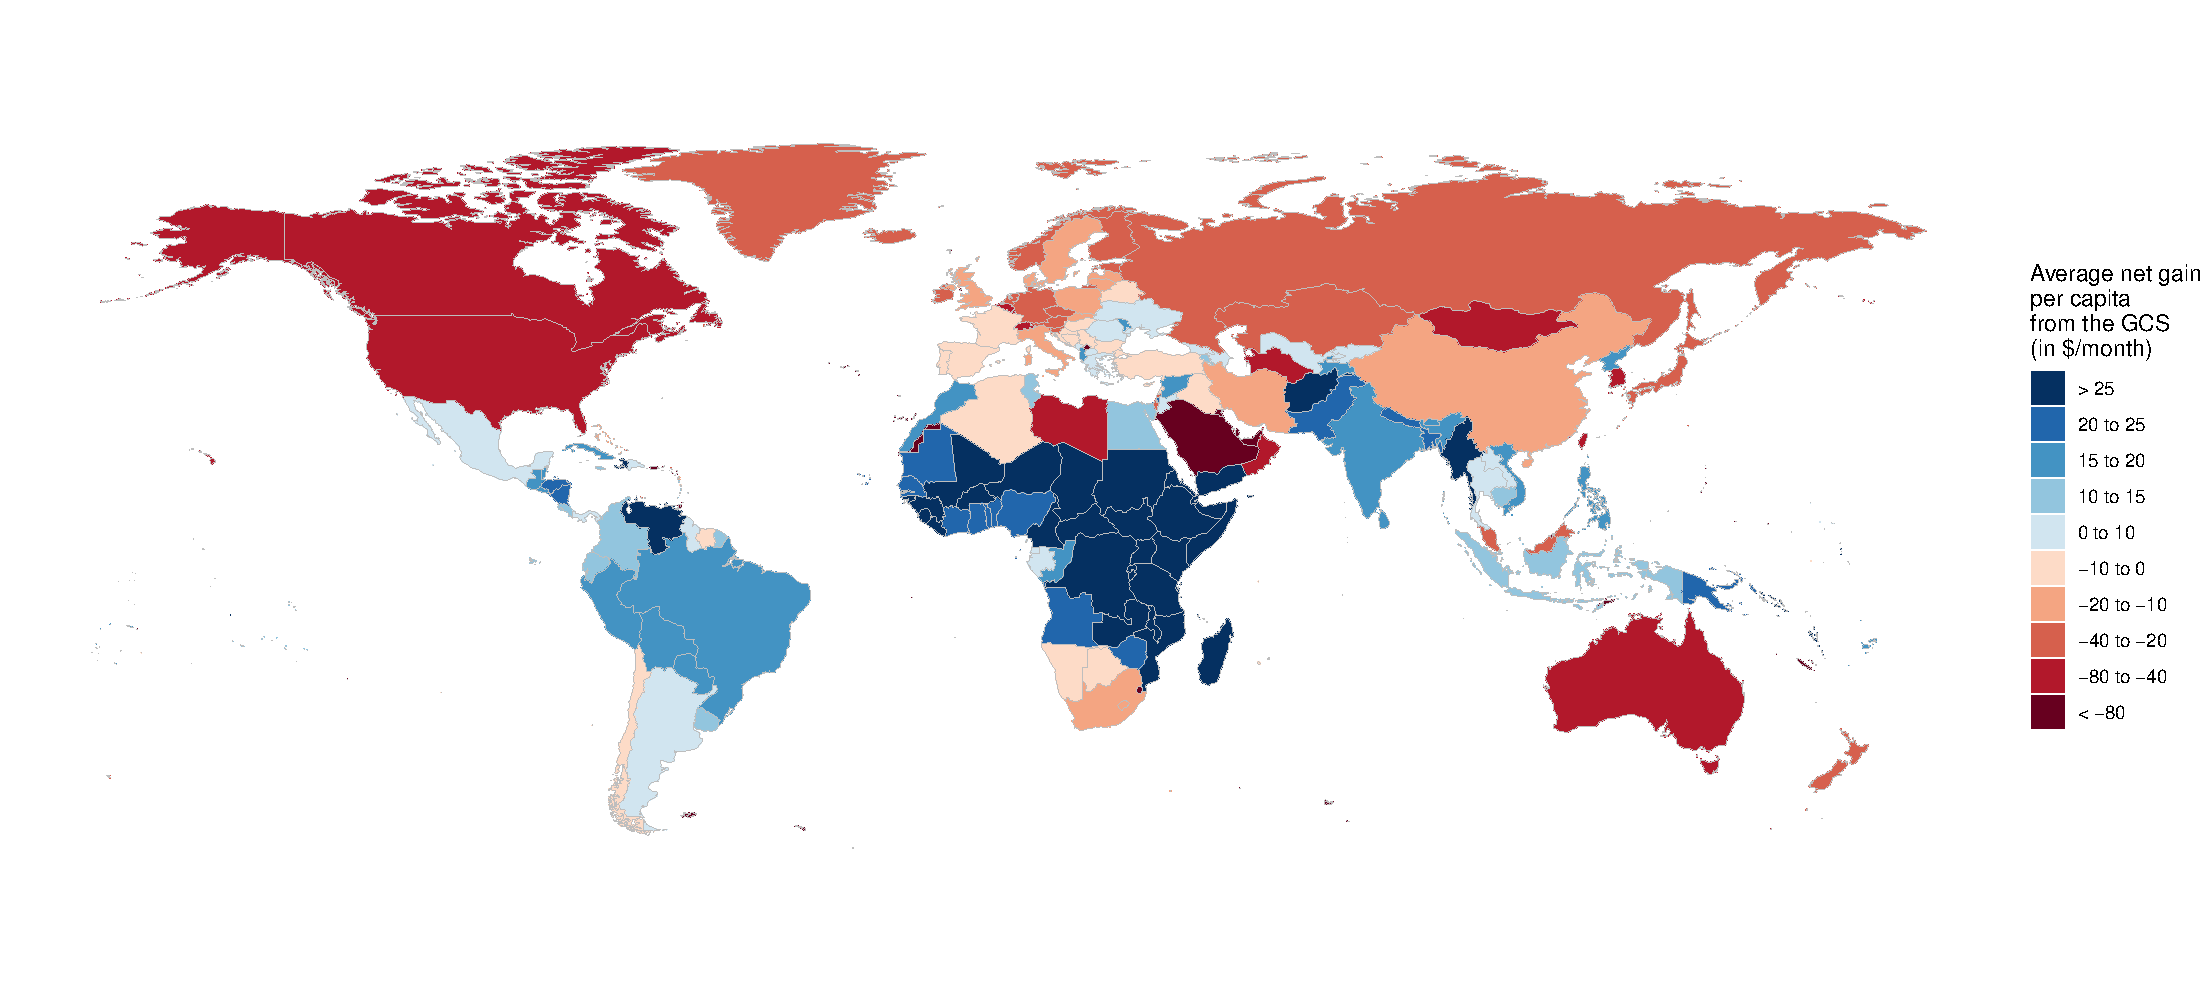
\includegraphics[height=.6\textheight]{../figures/maps/mean_gain_2030.pdf} 
    \end{figure}        
\end{frame}
\begin{frame}
\frametitle{GCS: presentation (3/3)}

\begin{itemize}
\setlength\itemsep{0.2cm}
    \item We present it to respondents as a club mechanism:
    \begin{itemize}
        \item[\ding{226}] ``The policy could be put in place as soon as countries totaling more than 60\% of global emissions agree on it. Countries that would refuse to take part in the policy could face sanctions (like tariffs) from the rest of the World and would be excluded from the basic income.''% TODO: check where this 60% comes from
    \end{itemize}

    \pause

    \item We make distributional effects salient, e.g., in US surveys:
    \begin{itemize}
        \item[\ding{226}] ``Each adult in the world would receive \$30/month per month, thereby lifting out of extreme poverty the 700 million people who earn less than \$2/day.''
        \item[\ding{226}] ``The typical American would lose out financially \$85 per month (as he or she would face \$115 per month in price increases, which is higher than the \$30 they would receive).''
    \end{itemize}

    \pause

    \item To check understanding, we ask respondents whether fellow citizens or the poorest humans would win/lose, provide correct answers, and randomly reward good responses.
\end{itemize}

\end{frame}
\begin{frame}
\frametitle{Complementary policies}

We want to study whether people approve more/less the GCS conditional on other measures being implemented. \pause We introduce:

\vspace{0.2cm}

\begin{itemize}
\setlength\itemsep{0.2cm}
    \item a National Redistribution Scheme (NR):
    \begin{itemize}
        \item[\ding{226}] this policy would increase taxes on the top [5\% in the US, 1\% in Eu) and provide cash transfers to all adults;
        \item[\ding{226}] for each country, policy calibrated so that cash transfer is equivalent to average net loss from the GCS;
        \item[\ding{226}] again, we ask comprehension question to check this is understood.
    \end{itemize}

    \pause

    \item a National Climate Policy (C):
    \begin{itemize}
        \item[\ding{226}] coal exit in the US;
        \item[\ding{226}] thermal insulation plan in Europe.
    \end{itemize}

    \pause

    \item a societal policy (used for the list experiment):
    \begin{itemize}
        \item[\ding{226}] marriage only for opposite-sex couples in the US;
        \item[\ding{226}] death penalty for major crimes in Europe.
    \end{itemize}
\end{itemize}

% TOSAY: explain why interacting them with the GCS matters.]

\end{frame}
\begin{frame}
\frametitle{Support for GCS and other policies}

\begin{figure}[h!]
    \caption[Support for the Global Climate Scheme]{Support for the GCS, NR and the combination of GCS, NR and C.}\label{fig:support_binary}
    \makebox[\textwidth][c]{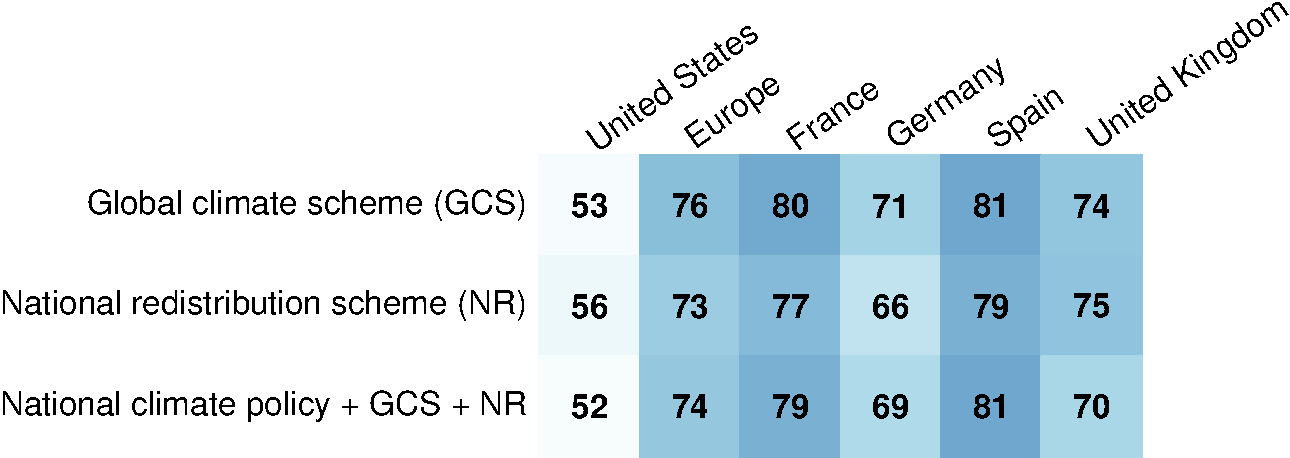
\includegraphics[width=0.9\textwidth]{../figures/country_comparison/support_binary_positive.pdf}} 
\end{figure}

\begin{itemize}
\setlength\itemsep{0.2cm}
    \item[\ding{226}] Majority support for the GCS in all countries: 54\% in US, 76\% in European countries.

    \item[\ding{226}] Similar level of support for NR.

    \item[\ding{226}] Similar level of support for combinaition of GCS, NR, C.
\end{itemize}

\end{frame}
\begin{frame}

\begin{table}[h]\label{tab:gcs_determinant}
    \caption[Determinants of support for the GCS]{Determinants of support for the Global Climate Scheme.} 
    \makebox[\textwidth][c]{
\resizebox*{!}{.93\textheight}{ % 73 is the max when there is a title
        
\begin{tabular}{@{\extracolsep{5pt}}lcccccc} 
\\[-1.8ex]\hline 
\hline \\[-1.8ex] 
 & \multicolumn{6}{c}{\makecell{Supports the Global Climate Scheme}} \\ 
\cline{2-7} 
\\[-1.8ex] & All & United States & France & Germany & United Kingdom & Spain \\ 
\hline \\[-1.8ex] 
 Country: ES & 0.113$^{***}$ &  &  &  &  &  \\ 
  & (0.023) &  &  &  &  &  \\ 
  Country: FR & 0.157$^{***}$ &  &  &  &  &  \\ 
  & (0.022) &  &  &  &  &  \\ 
  Country: UK & 0.078$^{***}$ &  &  &  &  &  \\ 
  & (0.023) &  &  &  &  &  \\ 
  Country: US & $-$0.218$^{***}$ &  &  &  &  &  \\ 
  & (0.017) &  &  &  &  &  \\ 
  Income quartile: 2 & 0.037$^{**}$ & 0.031 & 0.058 & 0.047 & 0.013 & 0.023 \\ 
  & (0.017) & (0.022) & (0.049) & (0.043) & (0.053) & (0.043) \\ 
  Income quartile: 3 & 0.042$^{**}$ & 0.033 & 0.059 & 0.080$^{**}$ & 0.074 & $-$0.052 \\ 
  & (0.017) & (0.024) & (0.052) & (0.040) & (0.056) & (0.052) \\ 
  Income quartile: 4 & 0.056$^{***}$ & 0.062$^{**}$ & $-$0.015 & 0.018 & $-$0.001 & $-$0.005 \\ 
  & (0.018) & (0.026) & (0.055) & (0.047) & (0.056) & (0.057) \\ 
  Diploma: Post secondary & 0.023$^{*}$ & 0.032$^{*}$ & 0.045 & 0.007 & 0.007 & $-$0.010 \\ 
  & (0.012) & (0.017) & (0.039) & (0.029) & (0.039) & (0.039) \\ 
  Age: 25-34 & $-$0.076$^{***}$ & $-$0.084$^{***}$ & $-$0.077 & $-$0.031 & $-$0.050 & $-$0.103 \\ 
  & (0.025) & (0.031) & (0.083) & (0.057) & (0.066) & (0.091) \\ 
  Age: 35-49 & $-$0.101$^{***}$ & $-$0.109$^{***}$ & $-$0.009 & $-$0.094$^{*}$ & $-$0.168$^{**}$ & $-$0.050 \\ 
  & (0.024) & (0.030) & (0.077) & (0.055) & (0.070) & (0.090) \\ 
  Age: 50-64 & $-$0.137$^{***}$ & $-$0.165$^{***}$ & $-$0.020 & $-$0.039 & $-$0.146$^{**}$ & $-$0.017 \\ 
  & (0.024) & (0.030) & (0.082) & (0.056) & (0.067) & (0.087) \\ 
  Age: 65+ & $-$0.116$^{***}$ & $-$0.142$^{***}$ & $-$0.045 & 0.003 & $-$0.258$^{***}$ & 0.011 \\ 
  & (0.028) & (0.034) & (0.094) & (0.076) & (0.091) & (0.105) \\ 
  Gender: Man & 0.019$^{*}$ & 0.022 & $-$0.018 & $-$0.014 & 0.042 & $-$0.005 \\ 
  & (0.011) & (0.015) & (0.033) & (0.029) & (0.038) & (0.034) \\ 
  Lives with partner & 0.029$^{**}$ & 0.023 & 0.082$^{**}$ & 0.070$^{**}$ & 0.017 & 0.040 \\ 
  & (0.013) & (0.017) & (0.038) & (0.033) & (0.038) & (0.039) \\ 
  Employment status: Retired & $-$0.020 & $-$0.046 & 0.096 & 0.087 & 0.040 & 0.001 \\ 
  & (0.024) & (0.030) & (0.075) & (0.081) & (0.082) & (0.073) \\ 
  Employment status: Student & 0.045 & 0.062 & 0.192$^{**}$ & 0.165$^{*}$ & 0.116 & $-$0.021 \\ 
  & (0.033) & (0.048) & (0.087) & (0.085) & (0.074) & (0.107) \\ 
  Employment status: Working & $-$0.016 & $-$0.020 & 0.006 & 0.082 & $-$0.050 & 0.036 \\ 
  & (0.019) & (0.024) & (0.056) & (0.064) & (0.056) & (0.051) \\ 
  Vote: Center-right or Right & $-$0.331$^{***}$ & $-$0.435$^{***}$ & $-$0.004 & $-$0.131$^{***}$ & $-$0.114$^{***}$ & $-$0.081$^{**}$ \\ 
  & (0.013) & (0.017) & (0.044) & (0.035) & (0.038) & (0.041) \\ 
  Vote: PNR/Non-voter & $-$0.184$^{***}$ & $-$0.198$^{***}$ & $-$0.034 & $-$0.196$^{***}$ & $-$0.116$^{**}$ & $-$0.108$^{***}$ \\ 
  & (0.016) & (0.022) & (0.043) & (0.039) & (0.046) & (0.040) \\ 
  Vote: Far right & $-$0.396$^{***}$ &  & $-$0.168$^{***}$ & $-$0.493$^{***}$ & $-$0.130 & $-$0.314$^{***}$ \\ 
  & (0.032) &  & (0.051) & (0.064) & (0.102) & (0.080) \\ 
  Urban & 0.049$^{***}$ & 0.072$^{***}$ & 0.019 & $-$0.002 & $-$0.014 & 0.017 \\ 
  & (0.012) & (0.018) & (0.032) & (0.029) & (0.036) & (0.033) \\ 
  Race: White &  & $-$0.030 &  &  &  &  \\ 
  &  & (0.019) &  &  &  &  \\ 
  Region: Northeast &  & 0.010 &  &  &  &  \\ 
  &  & (0.023) &  &  &  &  \\ 
  Region: South &  & 0.006 &  &  &  &  \\ 
  &  & (0.020) &  &  &  &  \\ 
  Region: West &  & 0.010 &  &  &  &  \\ 
  &  & (0.022) &  &  &  &  \\ 
  Swing State &  & $-$0.038$^{**}$ &  &  &  &  \\ 
  &  & (0.019) &  &  &  &  \\ 
 \hline \\[-1.8ex] 
Constant & 0.891 & 0.736 & 0.732 & 0.7 & 0.935 & 0.886 \\ 
Observations & 7,986 & 4,992 & 727 & 977 & 748 & 542 \\ 
R$^{2}$ & 0.160 & 0.181 & 0.067 & 0.116 & 0.043 & 0.063 \\ 
\hline 
\hline \\[-1.8ex] 
\textit{Note:}  & \multicolumn{6}{r}{$^{*}$p$<$0.1; $^{**}$p$<$0.05; $^{***}$p$<$0.01} \\ 
\end{tabular} 
        }
    }
    {\footnotesize %\textit{Note}: 
    }
\end{table}
    
\end{frame}
\begin{frame}
\frametitle{Attitudes towards other climate and redistributive policies}\label{slide_attitude_other_pol}

Among other results, we find that:

\vspace{0.2cm}

\begin{itemize}
\setlength\itemsep{0.3cm}
    \item most climate or redistributive policies we suggest are supported;
    
    \hyperlink{slide_support_other}{\beamergotobutton{Results}}
    
    \item high support for global tax on millionaires to finance low-income countries;
    \item majorities wish to devote significant part of the proceeds of a tax on top wealth (above 5m\$) to finance low-income countries; \hyperlink{slide_wealth_tax}{\beamergotobutton{Results}}
    \item people over-estimate foreign aid, but still want to increase it. \hyperlink{slide_foreign_aid_1}{\beamergotobutton{Results support}} \hyperlink{slide_foreign_aid_2}{\beamergotobutton{Results conditions 1}} \hyperlink{slide_foreign_aid_3}{\beamergotobutton{Results conditions 2}}
\end{itemize}

\vspace{0.3cm}
\pause

$\Rightarrow$ Overall, large stated support for global redistributive climate policies. \textbf{Is it sincere?}

\end{frame}

\section{Robustness and sincerity}

\begin{frame}[noframenumbering,plain]
\begin{center}
\huge Robustness and sincerity of support
\end{center}
\end{frame}

\begin{frame}
\frametitle{Petition}

    \begin{figure}
        \centering 
        \caption{Would you be willing to sign a petition for the [GCS / NR]? \\As soon as the survey is complete, we will send the results to the [head of state] (...) \textit{Yes/No} % U.S. President's office %, informing him what share of American people are willing to endorse the Global climate scheme. (You will NOT be asked to sign, only your answer here is required and remains anonymous.)
        }
        \vspace{-.2cm}
        \pause
        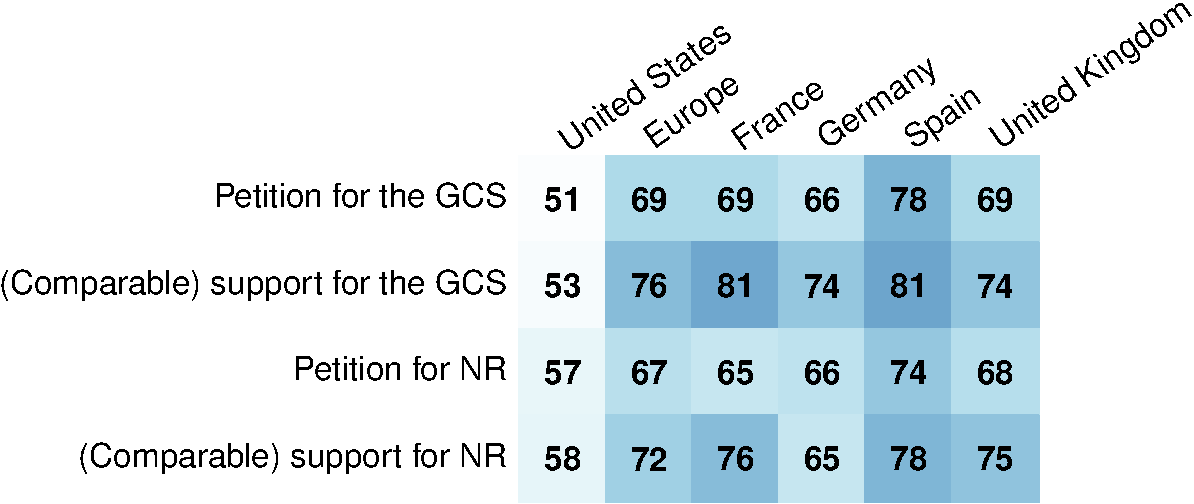
\includegraphics[height=.4\textheight]{../figures/country_comparison/petition_comparable_positive.pdf} 
    \end{figure}

$\Rightarrow$ Willingness to sign a real-stake petition is generally 1 to 7 p.p. lower than stated support. But not specific to GCS, and majorities are still willing to sign the petition.

\end{frame}

\begin{frame}
\frametitle{List experiment: design}

Basic idea:

\vspace{0.2cm}

\begin{itemize}
\setlength\itemsep{0.2cm}
    \item provide a list of policies;
    \item ask respondents \textit{how many} they support, without specifying which ones;
    \item randomly vary the content of the list across respondents;
    \item tacit support for a given policy is estimated as the effect of including that policy in a list on the number of policies supported.
\end{itemize}

\vspace{0.4cm}

Popular technique to reveal social desirability bias or silencing (e.g., on racism in the Southern U.S. (\textcolor{blue}{Kuklinski et al., 1997}) or opposition to the invasion of Ukraine in Russia (\textcolor{blue}{Chapkovski \& Schaub, 2022})).

\vspace{0.5cm}

In our case: list may include GCS, NR, C, and our societal policy.

\end{frame}
\begin{frame}
\frametitle{List experiment: results}

\begin{table}[h]
  \caption[List experiment: tacit support for the GCS]{Number of supported policies in the list experiment depending on the presence of the Global Climate Scheme (GCS) in the list.
  }\label{tab:list_exp}
  \makebox[\textwidth][c]{
\resizebox*{!}{.45\textwidth}{
\begin{tabular}{@{\extracolsep{5pt}}lccc} 
\\[-1.8ex]\hline 
\hline \\[-1.8ex] 
 & \multicolumn{3}{c}{Number of supported policies} \\ 
\cline{2-4} 
\\[-1.8ex] & All & US & Europe \\ 
\hline \\[-1.8ex] 
 List contains: GCS & 0.624$^{***}$ & 0.524$^{***}$ & 0.724$^{***}$ \\ 
  & (0.028) & (0.041) & (0.036) \\ 
\hline  \\[-1.8ex] \textit{Support for GCS} & 0.65  &  0.542  &  0.757 \\
\textit{Social desirability bias} & \textit{$ -0.026 $} & \textit{$ -0.018 $} & \textit{$ -0.033 $}\\
\textit{80\% C.I. for the bias} & \textit{ $[ -0.06 ; 0.01 ]$ } & \textit{ $[ -0.07 ; 0.01 ]$} & \textit{ $[ -0.08 ; 0.01 ]$}\\
 \hline \\[-1.8ex] 
Constant & 1.317 & 1.147 & 1.486 \\ 
Observations & 6,000 & 3,000 & 3,000 \\ 
R$^{2}$ & 0.089 & 0.065 & 0.125 \\ 
\hline 
\hline \\[-1.8ex] 
\textit{Note:}  & \multicolumn{3}{r}{$^{*}$p$<$0.1; $^{**}$p$<$0.05; $^{***}$p$<$0.01} \\ 
\end{tabular} 
  }}
\end{table}

$\Rightarrow$ Consistent with stated support, no evidence of social desirability bias.

% \makebox[\textwidth][c]{
% \resizebox*{!}{.93\textwidth}{ % 73 is the max when there is a title
%         
\begin{tabular}{@{\extracolsep{5pt}}lccc} 
\\[-1.8ex]\hline 
\hline \\[-1.8ex] 
 & \multicolumn{3}{c}{Number of supported policies} \\ 
\cline{2-4} 
\\[-1.8ex] & All & US & Europe \\ 
\hline \\[-1.8ex] 
 List contains: GCS & 0.624$^{***}$ & 0.524$^{***}$ & 0.724$^{***}$ \\ 
  & (0.028) & (0.041) & (0.036) \\ 
\hline  \\[-1.8ex] \textit{Support for GCS} & 0.65  &  0.542  &  0.757 \\
\textit{Social desirability bias} & \textit{$ -0.026 $} & \textit{$ -0.018 $} & \textit{$ -0.033 $}\\
\textit{80\% C.I. for the bias} & \textit{ $[ -0.06 ; 0.01 ]$ } & \textit{ $[ -0.07 ; 0.01 ]$} & \textit{ $[ -0.08 ; 0.01 ]$}\\
 \hline \\[-1.8ex] 
Constant & 1.317 & 1.147 & 1.486 \\ 
Observations & 6,000 & 3,000 & 3,000 \\ 
R$^{2}$ & 0.089 & 0.065 & 0.125 \\ 
\hline 
\hline \\[-1.8ex] 
\textit{Note:}  & \multicolumn{3}{r}{$^{*}$p$<$0.1; $^{**}$p$<$0.05; $^{***}$p$<$0.01} \\ 
\end{tabular} 
%   }

\end{frame}
% \begin{frame}
% \frametitle{List experiment: takeaway}
    
% \end{frame}
\begin{frame}
\frametitle{Conjoint analysis: design (1/2)}

\begin{itemize}
\setlength\itemsep{0.4cm}
    \item We run several conjoint analyses: people must choose between two alternative political platforms.

    \item We are interested in two main things: \vspace{0.2cm}
    \begin{itemize}
    \setlength\itemsep{0.2cm}
        \item[\ding{226}] How would campaining for the GCS affect a progressive candidate relative to a conservative candidate?

        \item[\ding{226}] How would campaining for the GCS affect a progressive candidate relative to another progressive candidate?
    \end{itemize}
\end{itemize}

\vspace{0.5cm}

$\Rightarrow$ We can use the conjoint analysis to implicitly reveal support for the GCS (and other policies), as well as how it interacts with other aspects of the political agenda.

\end{frame}
\begin{frame}
\frametitle{Conjoint analysis: design (2/2)}

\begin{figure}[h!]
    \caption[Choice between a conservative platform and a progressive platform with/without the GCS]{Choice between a conservative platform and a progressive platform with/without the GCS.}
    \vspace{-0.2cm}
    \makebox[\textwidth][c]{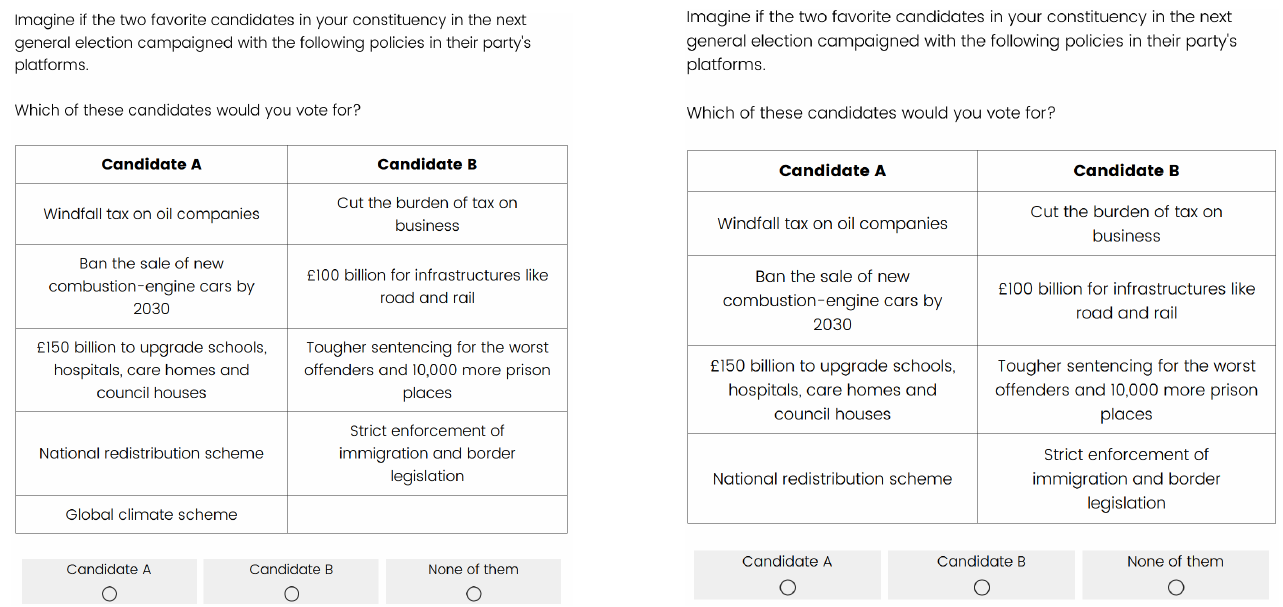
\includegraphics[width=1.0\textwidth]{../figures/conjoint_analysis_design.png}} 
\end{figure}


\end{frame}
\begin{frame}
\frametitle{Conjoint analysis: results (1/2)}

\begin{table} % NCCcomment [h]
  % MAJOR figure
  \caption[Influence of the GCS on electoral prospects]{Preference for a progressive platform depending on whether it includes the GCS or not.}
  \makebox[\textwidth][c]{
\resizebox*{!}{.25\textwidth}{
\begin{tabular}{@{\extracolsep{5pt}}lcccccc} 
\\[-1.8ex]\hline 
\hline \\[-1.8ex] 
 & \multicolumn{6}{c}{Prefers the Progressive platform} \\ 
\cline{2-7} 
\\[-1.8ex] & All & United States & France & Germany & UK & Spain \\ 
\hline \\[-1.8ex] 
 GCS in Progressive platform & 0.028$^{*}$ & 0.029 & 0.112$^{***}$ & 0.015 & 0.008 & $-$0.015 \\ 
  & (0.014) & (0.022) & (0.041) & (0.033) & (0.040) & (0.038) \\ 
 \hline \\[-1.8ex] 
Constant & 0.623 & 0.604 & 0.55 & 0.7 & 0.551 & 0.775 \\ 
Observations & 5,202 & 2,619 & 605 & 813 & 661 & 504 \\ 
R$^{2}$ & 0.001 & 0.001 & 0.013 & 0.0003 & 0.0001 & 0.0003 \\ 
\hline 
\hline \\[-1.8ex] 
\end{tabular} 
}}\label{tab:conjoint_c}
  {\scriptsize \textit{Note:} Simple OLS model. The 14\% of \textit{None of them} answers have been excluded from the regression samples. GCS has no significant influence on them. $^{*}p<0.1$; $^{**} p<0.05$; $^{***} p<0.01$. 
  }
\end{table}

\vspace{0.3cm}

$\Rightarrow$ A progressive candidate would not lose votes by endorsing the GCS, and could even gain 11 p.p.*** in France.


\end{frame}
\begin{frame}
\frametitle{Conjoint analysis: results (2/2)}

% To assess the effect of the GCS on the chances of success of a progressive candidate at a primary election, 

\begin{itemize}
\setlength\itemsep{0.2cm}
    \item ``Imagine that a [Left or Center-left coalition wins the next elections]. Here are two possible platforms on which [the coalition] may campaign'' (...) ``Even if you do not support the [Left or Center-left], which of these platforms do you prefer?''

    \item Policies in each platform are randomly drawn from a pool of credible left/center-left policies.

    \item For each country, we refer to specific parties. For the US, framed as a vote at the primary elections, not asked to republicans.
\end{itemize}

\begin{figure}[h!]
    \caption[Influence of the GCS on preferred platform]{Influence of the GCS on preferred platform:\\ Preference for a random platform A that contains the Global Climate Scheme rather than a platform B that does not (in percent).}\label{fig:conjoint_left_ag_b}\vspace{-0.2cm}
    \makebox[\textwidth][c]{
\includegraphics[width=1.2\textwidth]{../figures/country_comparison/conjoint_left_ag_b_binary_positive.pdf}} 
\end{figure}

% Imagine that a [Left or Center-left coalition wins the next elections]. Here are two possible platforms on which
% [the coalition] may campaign (the policies in each platform are randomly drawn from a pool of credible
% [Left/Center-left] policies).
% Even if you do not support the Left, which of these platforms do you prefer?
% [FR: Left or center-left; DE: rot-rot-grüne; ES: PSOE; UK: Labour; US: Democratic primary (not asked to
% Republican)]

\end{frame}
\begin{frame}
\frametitle{Policy prioritization}

We also implement a prioritization task:

\vspace{0.1cm}

\begin{itemize}
\setlength\itemsep{0.1cm}
    \item respondents have 100 points to allocate to 6 policies;

    \item they are told that ``The more you give points to a policy, the more you support it.'';

    \item six policies are randomly drawn from a larger list;

    \item on average, policies get 16.7 pts when they are included.
\end{itemize}

\vspace{0.3cm}
\pause

Results:

\vspace{0.1cm}

\begin{itemize}
\setlength\itemsep{0.1cm}
    \item In each country, the GCS ranks in the middle of all policies or above, from 15.4 pts in the U.S. to 22.9 pts in Germany (2nd most prioritized after tax on millionaires).

    \item Global tax on millionaires consistently ranks near the top.

    \item Contrasts with ``ban the sale of new combustion-engine cars by 2030'', one of the least preferred (from 7.8 pts in France to 11.4 in the UK).
\end{itemize}


\end{frame}

\section{Additional results}

\begin{frame}[noframenumbering,plain]
\begin{center}
\huge Additional results
\end{center}
\end{frame}


\begin{frame}
\frametitle{Campaign effect}

\begin{itemize}
\setlength\itemsep{0.3cm}
    \item The campaign effect (cf. \textcolor{blue}{Anderson et al, 2023}) refers to the drop in support policies may experience after entering the public debate.

    \item To simulate this effect, we expose a sub-sample of the US survey to a list of pros and cons about the GCS \textit{before} asking for their approval.

    \pause

    \item We observe a decrease in support by 11 p.p.:
    \begin{itemize}
        \item[\ding{226}] some items may cast doubt about the feasibility/desirability of the policy (e.g., ``It could be subject to fraud'', ``It could fuel corruption in low-income countries'').
    \end{itemize}
\end{itemize}

\vspace{0.4cm}

$\Rightarrow$ Public support for the GCS (and other global policies) could be sensitive to campaigns against it!

\end{frame}
\begin{frame}
\frametitle{Second-order beliefs}

Question: ``According to you, what percentage of [country-fellow] answer Yes to the previous question? The three people who are closest to the true value get \$50.'' Mean answer:

\begin{figure}[h!]
    \caption[Beliefs about support vs actual support for the GCS and NR]{Beliefs regarding the support for the GCS and NR.}\label{fig:belief}
    \vspace{-0.3cm}
    \makebox[\textwidth][c]{
\includegraphics[width=1\textwidth]{../figures/country_comparison/belief_all_mean.pdf}} 
\end{figure}

$\Rightarrow$ No evidence of pluralistic ignorance in the US, some under-estimation in Europe but still, people expect majority support.

\end{frame}
\begin{frame}
\frametitle{Donation: design}

Do we observe universalistic values in behaviors?

\vspace{0.25cm}

\begin{itemize}
\setlength\itemsep{0.5cm}
    \item We ask questions about perceived importance of global issues, whose interests diplomats should defend in climate negotiations, etc.

    \item In addition, we design an incentivized donation:

    \begin{itemize}
    \setlength\itemsep{0.25cm}
        \item[\ding{226}] Respondents might win a \$100 (/\texteuro/\pounds) lottery prize, they have to decide which share to donate if they win.

        \item[\ding{226}] Donation is to people in need, either in Africa or in their own country (random treatment).
    \end{itemize}
\end{itemize}

\end{frame}
\begin{frame}
\frametitle{Donation: results}

\begin{table}[h]\label{tab:donation}\vspace*{-.35cm}
        \caption{(...) In case you are winner of the lottery, what share of the [\$]100 would you donate to [African / [own country]] people living in poverty through GiveDirectly?} 
        \makebox[\textwidth][c]{\resizebox*{!}{.35\textwidth}{
\begin{tabular}{@{\extracolsep{5pt}}lcccc} 
\\[-1.8ex]\hline 
\hline \\[-1.8ex] 
 & \multicolumn{4}{c}{Donation to poor people (in \%)} \\ 
\cline{2-5} 
\\[-1.8ex] & All & US & US & Eu \\ 
\hline \\[-1.8ex] 
 Poor is in own country & 0.590 & 2.509$^{**}$ & 0.046 & $-$1.349 \\ 
  & (0.799) & (1.152) & (1.691) & (1.108) \\ 
  Poor is in own country $\times$ Vote: \textit{not} Biden &  &  & 3.954$^{*}$ &  \\ 
  &  &  & (2.279) &  \\ 
 \hline \\[-1.8ex] 
Mean & 34.034 & 33.658 & 33.658 & 34.41 \\ 
Observations & 6,000 & 3,000 & 3,000 & 3,000 \\ 
R$^{2}$ & 0.0001 & 0.002 & 0.034 & 0.0005 \\ 
\hline 
\hline \\[-1.8ex] 
\end{tabular} }}
\end{table}

$\Rightarrow$ U.S. non-voters and Trump voters donate 4 p.p. more to fellow citizens, others give the same amount.

\end{frame}


\section{Conclusion}

\begin{frame}[noframenumbering,plain]
\begin{center}
\huge Conclusion
\end{center}
\end{frame}

\begin{frame}
\frametitle{Takeaways}

\begin{itemize}
\setlength\itemsep{0.2cm}
    \item High support for global climate and redistributive policies across the world:
    \begin{itemize}
    \setlength\itemsep{0.1cm}
        \item[\ding{226}] high international support for global carbon budget;
        \item[\ding{226}] consensus on the ``per capita'' allocation rule;
        \item[\ding{226}] majorities support global climate policies, including with transfers detrimental to their countries;
        \item[\ding{226}] most people favorable to increasing foreign aid, despite overestimating current levels.
    \end{itemize}

    \item This support appears mostly sincere:
    \begin{itemize}
    \setlength\itemsep{0.1cm}
        \item[\ding{226}] evidence from real-stake petitions, list experiment, prioritization task, and conjoint analysis suggest support for the GCS is not cheap talk;

        \item[\ding{226}] no evidence that a progressive candidate would lose vote shares by endorsing the GCS.
    \end{itemize}

\end{itemize}

\end{frame}
\begin{frame}
\frametitle{Discussion}

If people are sincere about the support for global climate and redistributive policies, how come are they not more prominent in the public debate?

\vspace{0.4cm}

Potential reasons:

\vspace{0.2cm}

\begin{itemize}
\setlength\itemsep{0.3cm}
    \item National bias in power structures (elections, media) and mental structures (hymns, sport teams)?

    \item Pluralistic ignorance of the elites?

    \item Ideas whose time has come, and just lack some advocacy?
\end{itemize}

\vspace{0.5cm}

$\Rightarrow$ More research needed on the topic!

\end{frame}

\section{Appendix}

\begin{frame}[noframenumbering,plain]
\begin{center}
\huge Appendix
\end{center}
\end{frame}

\begin{frame}
\frametitle{Wording policy questions}\label{slide_wording}

\begin{itemize}

    \item ``All countries have signed the Paris agreement that aims to contain global warming "well below +2°C". To limit global warming to this level, there is a maximum amount of greenhouse gases we can emit globally, called the carbon budget. Each country could aim to emit less than a share of the carbon budget. To respect the global carbon budget, countries that emit more than their national share would pay a fee to countries that emit less than their share. Do you support such a policy?''

    \item ``Do you support or oppose establishing a global democratic assembly whose role would be to draft international treaties against climate change? Each adult across the world would have one vote to elect members of the assembly.''

    \item ``Do you support or oppose a tax on all millionaires around the world to finance lowincome countries that comply with international standards regarding climate action? This would finance infrastructure and public services such as access to drinking water, healthcare, and education.''
\end{itemize}

\hyperlink{slide_global_support}{\beamerreturnbutton{Back}}

\end{frame}

\begin{frame}
\frametitle{Wealth tax}\label{slide_wealth_tax}

\begin{figure}
    \centering 
    \caption[Preferred share of wealth tax for low-income countries]{Percent of global wealth tax that should finance low-income countries (\textit{mean}).}
    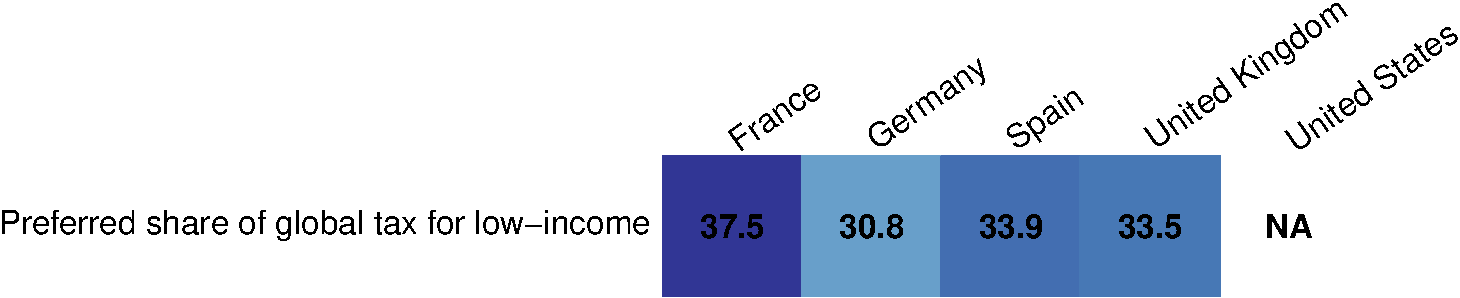
\includegraphics[width=1\textwidth]{../figures/country_comparison/global_tax_global_share_mean.pdf} \label{fig:global_share_mean}
\end{figure}

\hyperlink{slide_attitude_other_pol}{\beamerreturnbutton{Back}}
    
\end{frame}
\begin{frame}
\frametitle{Support: other global policies}\label{slide_support_other}

\begin{figure}
  \caption[Relative support for further global policies]{Relative support for various global policies (percentage of \textit{somewhat} or \textit{strong support}, after excluding \textit{indifferent} answers).}
  \vspace{-0.35cm}
  \makebox[\textwidth][c]{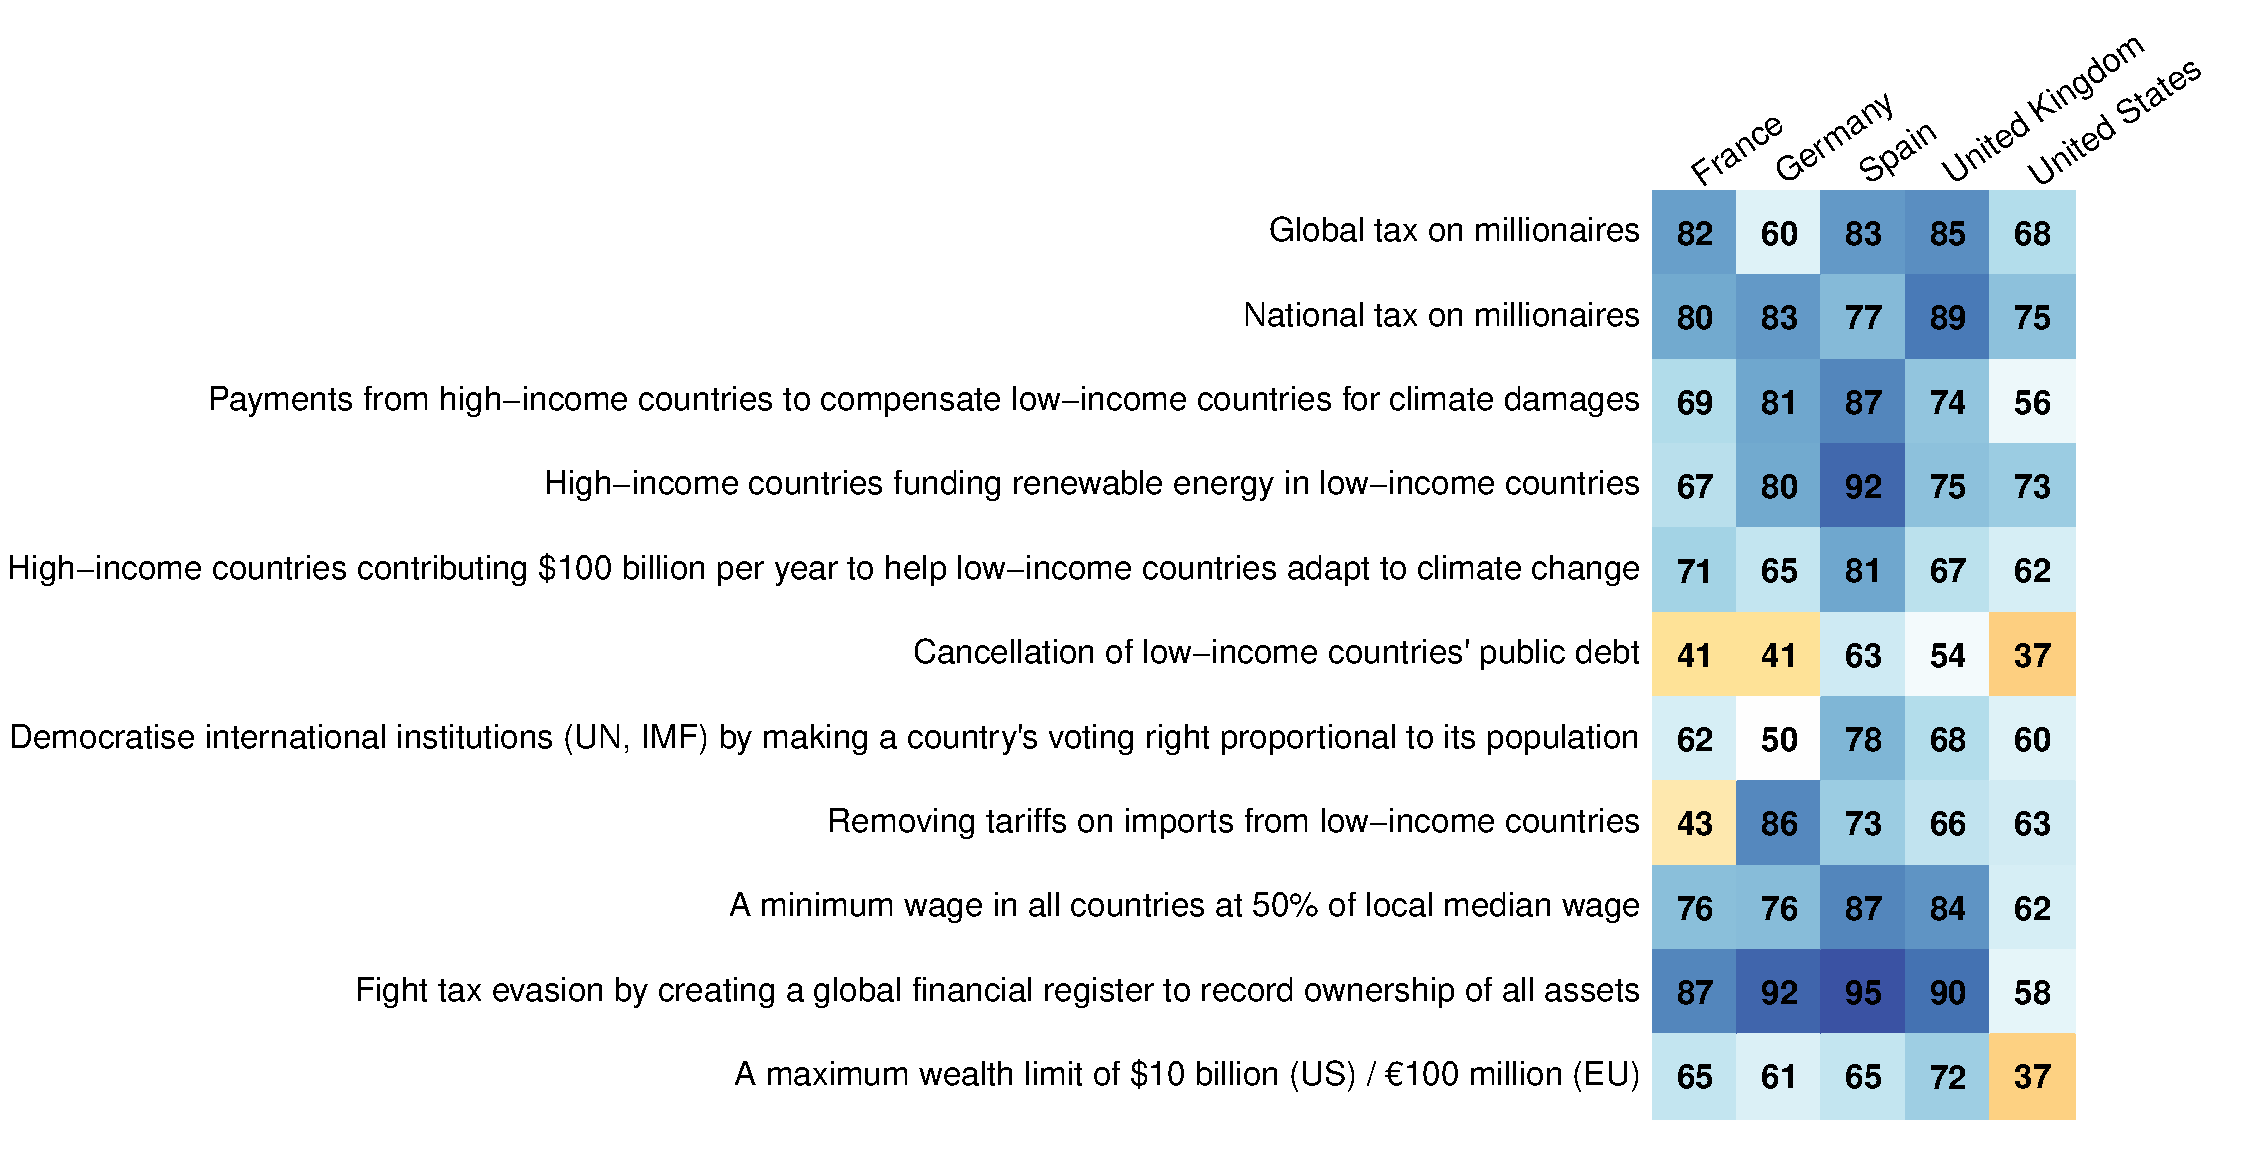
\includegraphics[width=.8\textwidth]{../figures/country_comparison/support_likert_share.pdf}}\label{fig:support}
\end{figure} 

\vspace{-0.7cm}
\hyperlink{slide_attitude_other_pol}{\beamerreturnbutton{Back}}
    
\end{frame}
\begin{frame}
\frametitle{Foreign aid (1/3)}\label{slide_foreign_aid_1}

\begin{figure}[h!]
  \caption[Attitudes on the evolution of foreign aid]{Attitudes regarding the evolution of [own country] foreign aid.}
  \makebox[\textwidth][c]{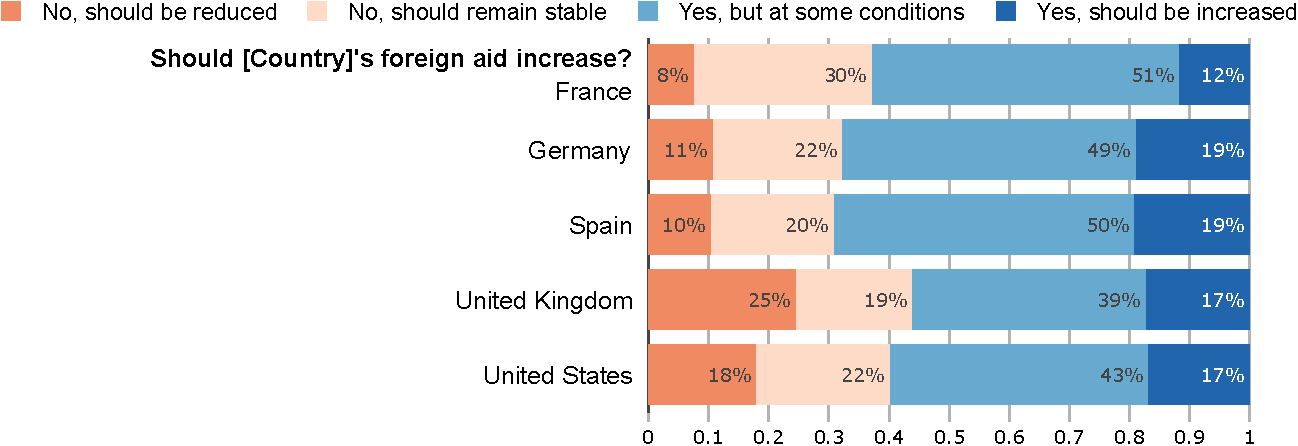
\includegraphics[width=1\textwidth]{../figures/country_comparison/foreign_aid_raise_support.pdf}} 
\end{figure}

\hyperlink{slide_attitude_other_pol}{\beamerreturnbutton{Back}}

\end{frame}
\begin{frame}
\frametitle{Foreign aid (2/3)}\label{slide_foreign_aid_2}

\begin{figure}[h!]
  \caption[Conditions at which foreign aid should be increased]{Conditions at which foreign aid should be increased (in percent). [Asked to those who wish an increase of foreign aid at some conditions.]}\label{fig:foreign_aid_condition}
  \makebox[\textwidth][c]{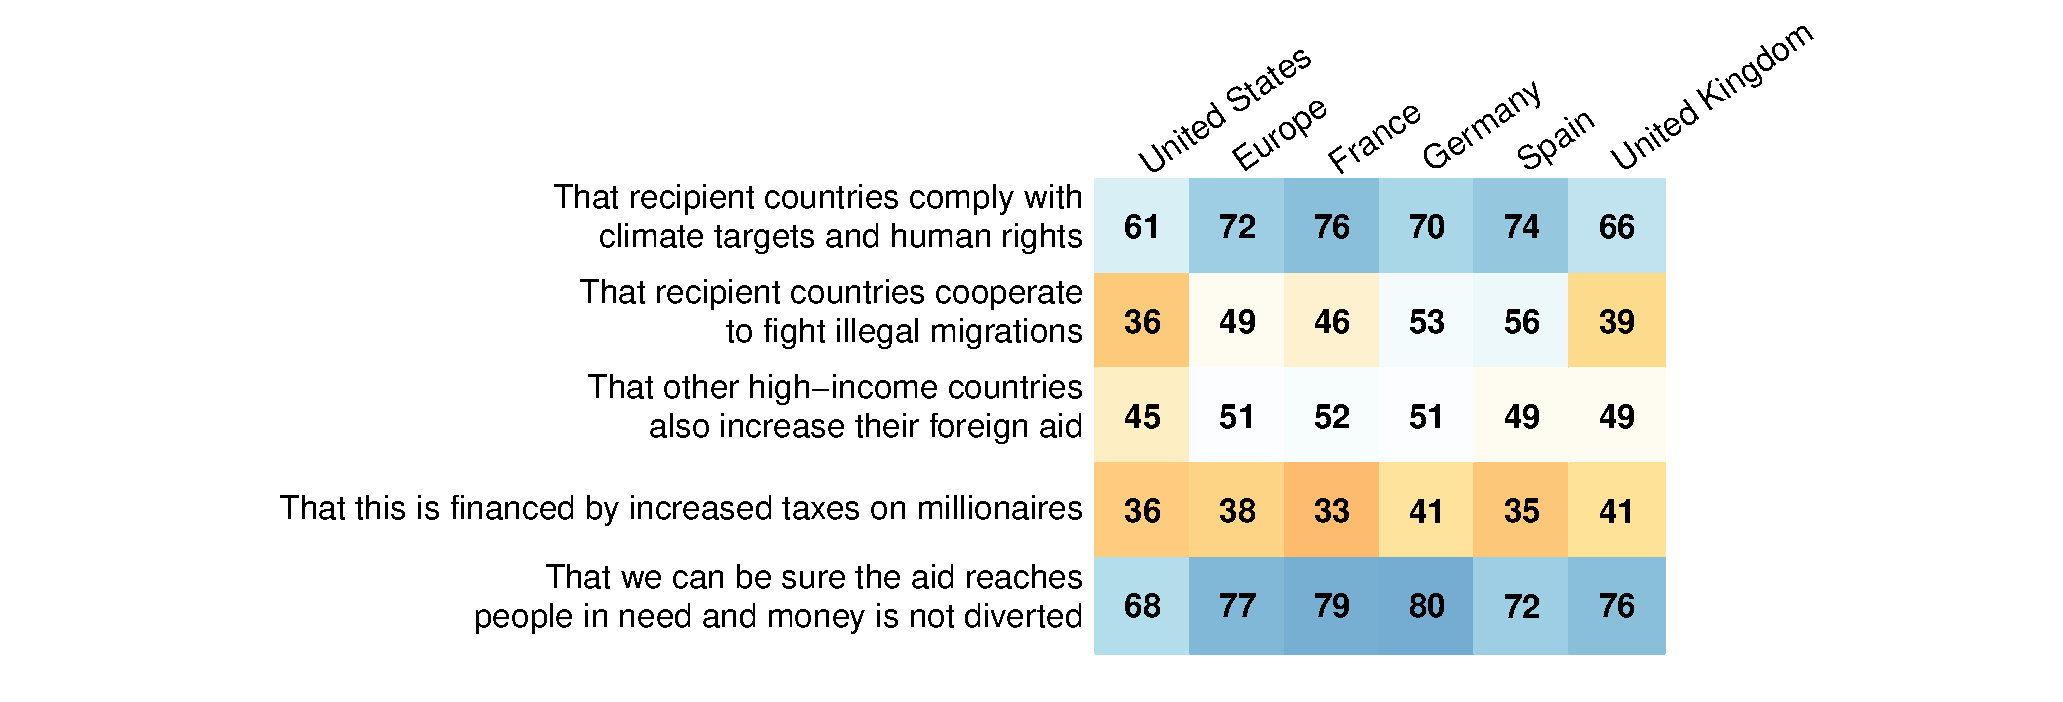
\includegraphics[width=1\textwidth]{../figures/country_comparison/foreign_aid_condition_positive.pdf}} 
\end{figure}

\hyperlink{slide_attitude_other_pol}{\beamerreturnbutton{Back}}

\end{frame}
\begin{frame}
\frametitle{Foreign aid (3/3)}\label{slide_foreign_aid_3}

\begin{figure}[h!]
  \caption[Reasons why foreign aid should not be increased]{Reasons why foreign aid should not be increased (in percent). [Asked to those who wish a decrease or stability of foreign aid.]}\label{fig:foreign_aid_no}
  \makebox[\textwidth][c]{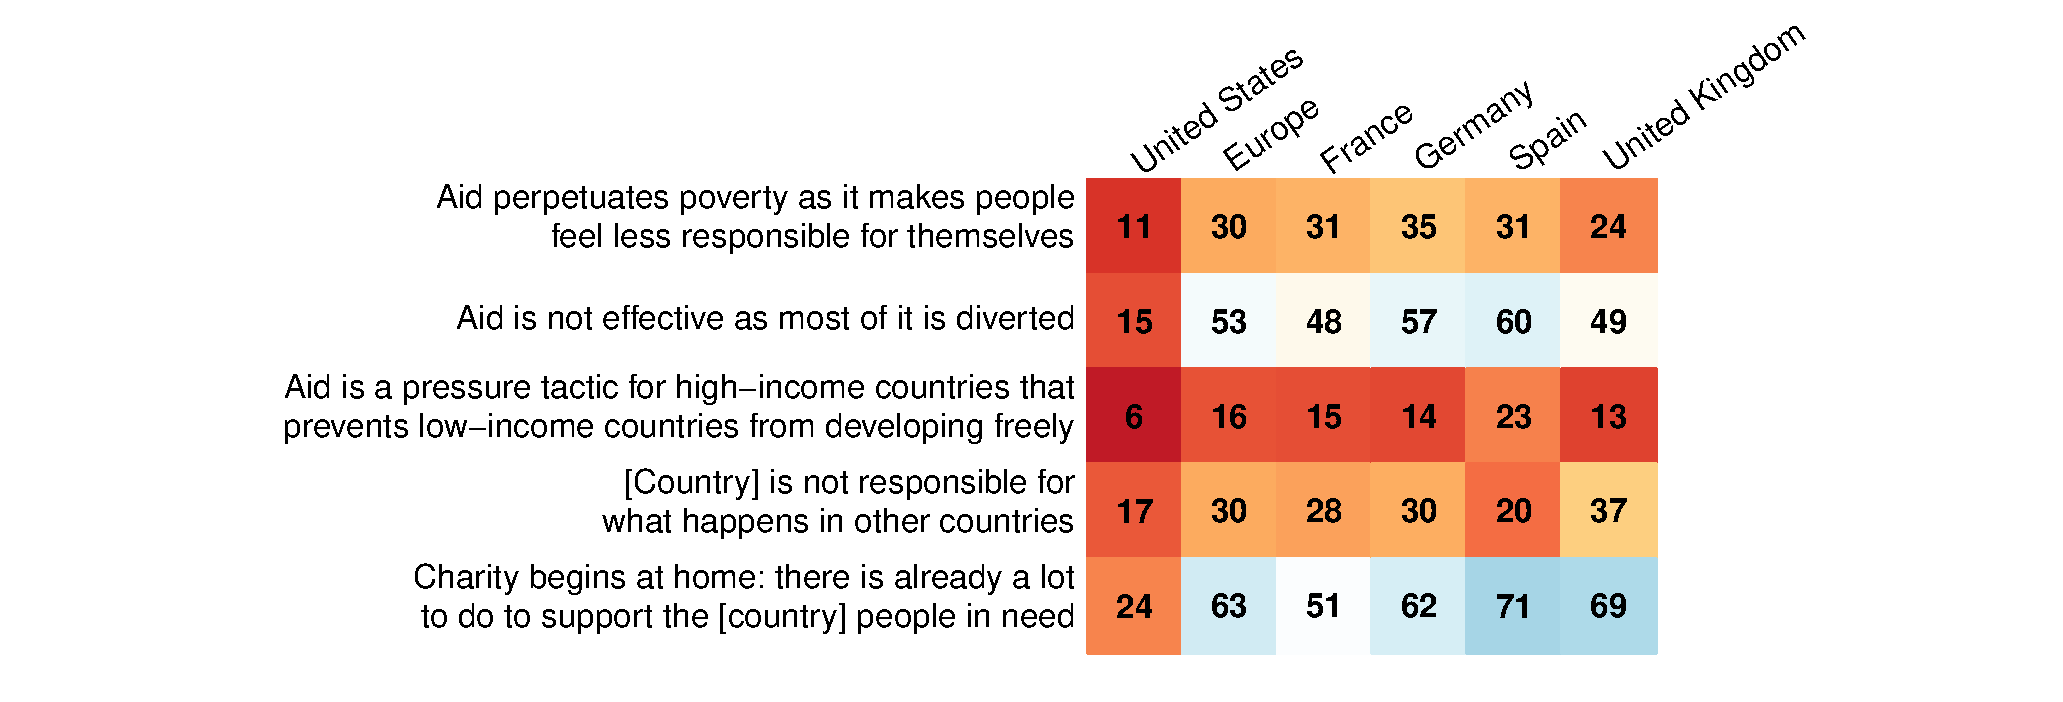
\includegraphics[width=1\textwidth]{../figures/country_comparison/foreign_aid_no_positive.pdf}} 
\end{figure}

\hyperlink{slide_attitude_other_pol}{\beamerreturnbutton{Back}}

\end{frame}


\end{document} 




